%%%%%%%%%%%%%%%%%%%%%%%%%%%%%%%%%%%%%%%%%%%%%%%%%%%%%%
%                                                    %
%        Modelo de Disserta��o para Gradua��o        %
%                                                    %
% Elabora��o  : Grupo PET-Tele                       %
% Respons�veis: Marcio Camoleze de Andrade           %
%               Thiago Muniz de Souza                %
% Orienta��o  : Prof. Alexandre Santos de la Vega    %
% Inicio: abr/2008                                   %
% Ultima modificacao: abr/2008                       %
%                                                    %
%%%%%%%%%%%%%%%%%%%%%%%%%%%%%%%%%%%%%%%%%%%%%%%%%%%%%%


\documentclass[a4paper,oneside]{book}

\pagestyle{myheadings}

%%%%%%%%%%%%%%%%%%%%%%%%%%%
% Pacotes para acentua��o %
%%%%%%%%%%%%%%%%%%%%%%%%%%%
\usepackage[utf8]{inputenc}
\usepackage[T1]{fontenc}
\usepackage{ae}

%%%%%%%%%%%

\usepackage[brazilian]{babel}

\usepackage{graphicx}
\usepackage{float}
\usepackage{amssymb}% http://ctan.org/pkg/amssymb
\usepackage{pifont}% http://ctan.org/pkg/pifont
\usepackage{booktabs,caption,fixltx2e}
\usepackage[flushleft]{threeparttable}
\usepackage[final]{pdfpages}

\newcommand{\cmark}{\ding{51}}%
\newcommand{\xmark}{\ding{55}}%

%%%%%%%%%%%

\linespread{1.5} % espa�amento entre linhas


%%%%%%%%%%%%%%%%%%%%%%%%%%%%%%%%%%%%%%%%%%%%%%%%%%%%%%
%              Formata��o da P�gina                  %
%%%%%%%%%%%%%%%%%%%%%%%%%%%%%%%%%%%%%%%%%%%%%%%%%%%%%%

% horizontal
\setlength{\hoffset}{-1in}

\setlength{\oddsidemargin}{3.0cm} 

\setlength{\textwidth}{160mm} % (210mm - 30mm - 20mm)

\setlength{\parindent}{1.25cm} % identa��o de cada par�grafo

% vertical
\setlength{\voffset}{-1in}
\addtolength{\voffset}{2.0cm}

\setlength{\topmargin}{0.0cm}

\setlength{\headheight}{5mm}
\setlength{\headsep}{5mm}

\setlength{\textheight}{247mm} % (297mm - 30mm - 20mm)

%\setlength{\footskip}{0mm}

%%%%%%%%%%%%%%%%%%%%%%%%%%%%%%%%%%%%%%%%%%%%%%%%%%%%%%


\begin{document}

\graphicspath{ {images/} }

%%%%%%%%%%%%%%%%%%%%%%%%%%%%%%%%%%%%%%%%%%%%%%%%%%%%%%
%                  Capa da Monografia                %
%%%%%%%%%%%%%%%%%%%%%%%%%%%%%%%%%%%%%%%%%%%%%%%%%%%%%%

\begin{titlepage}
  \begin{center}
    \Large{\textsc{Universidade Federal Fluminense} \\
           \textsc{Centro Tecnológico} \\ 
           \textsc{Instituto de Computação} \\
           \textsc{Curso de Sistemas de Informação} \\
            \textsc{Curso de Ciência da Computação}
          }
    \par\vfill
    \LARGE{IGOR BARBOSA PINTO}\\
    \LARGE{TIAGO CÂNDIDO ALMEIDA SANTOS}
    \par\vfill
%    \bigskip
    \LARGE{INTEGRA UFF - SISTEMA DE GESTÃO DE APRENDIZADO}
    \par\vfill
    \Large{Niterói-RJ\\2016}
  \end{center}
\end{titlepage}



%%%%%%%%%%%%%%%%%%%%%%%%%%%%%%%%%%%%%%%%%%%%%%%%%%%%%%
%                Numeracao em romano                 %
%%%%%%%%%%%%%%%%%%%%%%%%%%%%%%%%%%%%%%%%%%%%%%%%%%%%%%

\pagenumbering{roman}
\setcounter{page}{2}



%%%%%%%%%%%%%%%%%%%%%%%%%%%%%%%%%%%%%%%%%%%%%%%%%%%%%%
%                   Folha de Rosto                   %
%%%%%%%%%%%%%%%%%%%%%%%%%%%%%%%%%%%%%%%%%%%%%%%%%%%%%%


\begin{center}

IGOR BARBOSA PINTO\\
TIAGO CÂNDIDO ALMEIDA SANTOS

\vfill

INTEGRA UFF - SISTEMA DE GESTÃO DE APRENDIZADO

\vspace{3.0cm}

\begin{flushright}
\begin{minipage}{0.50\textwidth}

Monografia apresentada ao Departamento\linebreak
de Ciência da Computação da Universidade \linebreak
Federal Fluminense, como requisito parcial \linebreak
para obtenção do Grau de Bacharel em \linebreak
Ciência da Computação e \linebreak Bacharel de Sistemas de Informação.

\end{minipage}
\end{flushright}

\vspace{3.0cm}

Orientador: Prof. Dr. Raphael Pereira de Oliveira Guerra

\vfill

Niterói-RJ\\2016

\end{center}

\newpage

%%%%%%%%%%%%%%%%%%%%%%%%%%%%%%%%%%%%%%%%%%%%%%%%%%%%%%
%                 Folha de Aprovação                 %
%%%%%%%%%%%%%%%%%%%%%%%%%%%%%%%%%%%%%%%%%%%%%%%%%%%%%%

%\begin{center}

%SEU NOME EM LETRA MAIÚSCULA

%\vspace{1.0cm}

%TÍTULO DA MONOGRAFIA EM LETRA MAIÚSCULA

%\vspace{1.0cm}

%\begin{flushright}
%\begin{minipage}{0.45\textwidth}

%Dissertação apresentada ao Curso de Graduação \linebreak em Engenharia de Telecomunicações da \linebreak Universidade Federal Fluminense, como \linebreak requisito parcial para obtenção do Grau de ???. Área de Concentração: Sistemas de Telecomunicações.

%\end{minipage}
%\end{flushright}

%\vfill

%\begin{flushleft}

%Aprovada em MÊS de ANO.

%\end{flushleft}

%\vfill

%BANCA EXAMINADORA

%\vfill

%\hrulefill \\Prof. Dr. NOME DO ORIENTADOR EM LETRA MAIÚSCULA - Orientador\\UFF\\

%\vfill

%\hrulefill \\Prof. NOME DO PROFESSOR\\INSTITUIÇÃO\\

%\vfill

%\hrulefill \\Prof. NOME DO PROFESSOR\\INSTITUIÇÃO\\

%\vfill

%\hrulefill \\Prof. NOME DO PROFESSOR\\INSTITUIÇÃO\\

%\vfill

%Niterói-RJ\\Ano de conclusão do trabalho

%\end{center}

%\newpage

%%%%%%%%%%%%%%%%%%%%%%%%%%%%%%%%%%%%%%%%%%%%%%%%%%%%%%%%
%	               Dedicat�ria                     %
%%%%%%%%%%%%%%%%%%%%%%%%%%%%%%%%%%%%%%%%%%%%%%%%%%%%%%%%

\begin{flushright}
\begin{minipage}{0.5\textwidth}

\vspace{15.0cm} % espa�o do topo at� o in�cio da dedicat�ria 

"Existem apenas duas coisas dif�ceis em Ci�ncia da Computa��o: invalida��o de de cache e dar nome �s coisas." \\
(KARLTON, Phil)

\end{minipage}
\end{flushright}




%%%%%%%%%%%%%%%%%%%%%%%%%%%%%%%%%%%%%%%%%%%%%%%%%%%%%%%%
%	              Agradecimentos                   %
%%%%%%%%%%%%%%%%%%%%%%%%%%%%%%%%%%%%%%%%%%%%%%%%%%%%%%%%

\chapter*{Agradecimentos}
\addcontentsline{toc}{chapter}{Agradecimentos}

\thispagestyle{myheadings}

\noindent

Espa�o reservado para os agradecimentos.

Agradecimento 1.

Agradecimento 2.

...

Agradecimento N.

Os agradecimentos devem ser sucintos e espec�ficos
a cada tipo de ajuda, a cada id�ia relevante, 
a cada empr�stimo significativo, pois um agradecimento
�, de certa forma, um cr�dito dado a algu�m \cite{norma:esjo2005}.



%%%%%%%%%%%%%%%%%%%%%%%%%%%%%%%%%%%%%%%%%%%%%%%%%%%%%%%%
%                  Lista de Ilustra��es                %
%%%%%%%%%%%%%%%%%%%%%%%%%%%%%%%%%%%%%%%%%%%%%%%%%%%%%%%%

\listoffigures
\addcontentsline{toc}{chapter}{Lista de Figuras}

\thispagestyle{myheadings}



%%%%%%%%%%%%%%%%%%%%%%%%%%%%%%%%%%%%%%%%%%%%%%%%%%%%%%%%
%                   Lista de Tabelas                   %
%%%%%%%%%%%%%%%%%%%%%%%%%%%%%%%%%%%%%%%%%%%%%%%%%%%%%%%%

\listoftables
\addcontentsline{toc}{chapter}{Lista de Tabelas}

\thispagestyle{myheadings}


%%%%%%%%%%%%%%%%%%%%%%%%%%%%%%%%%%%%%%%%%%%%%%%%%%%%%%%%
%                   Lista de Siglas                   %
%%%%%%%%%%%%%%%%%%%%%%%%%%%%%%%%%%%%%%%%%%%%%%%%%%%%%%%%

\chapter*{Lista de Abreviaturas e Siglas}
\addcontentsline{toc}{chapter}{Lista de Abreviaturas e Siglas}

\thispagestyle{myheadings}

\begin{description}
    \item [API:] \textit{Application Programming Interface}
    \item [SGA:] Sistema de Gestão de Aprendizagem
    \item [AVA:] Ambiente Virtual de Aprendizagem
    \item [CVDS:] Ciclo de Vida de Desenvolvimento de Sistemas
    \item [TDD:] \textit{Test-driven Development}
    \item [XP:] \textit{Extreme Programming}
    \item [LMS:] \textit{Learning Management System}
    \item [UFF:] Universidade Federal Fluminense
    \item [COC:] \textit{Convention Over Configuration}
    \item [URL:] \textit{Uniform Resource Locator}
    \item [REST:] \textit{Representational State Transfer}
    \item [TFD:] \textit{Test-First Development}
    \item [MVC:] Modelo-Visão-Controlador
    \item [HTTP:] \textit{Hypertext Transfer Protocol}
    \item [HTML:] \textit{Hypertext Markup Language}
    \item [JSON:] \textit{JavaScript Object Notation}
    \item [CSS:] \textit{Cascading Style Sheets}
    \item [GPA:] \textit{Grade Point Average}
\end{description}



%%%%%%%%%%%%%%%%%%%%%%%%%%%%%%%%%%%%%%%%%%%%%%%%%%%%%%%%
%                       Sum�rio                        %
%%%%%%%%%%%%%%%%%%%%%%%%%%%%%%%%%%%%%%%%%%%%%%%%%%%%%%%%

\tableofcontents

\thispagestyle{myheadings}




%%%%%%%%%%%%%%%%%%%%%%%%%%%%%%%%%%%%%%%%%%%%%%%%%%%%
%            Resumo na l�ngua vern�cula            %
%%%%%%%%%%%%%%%%%%%%%%%%%%%%%%%%%%%%%%%%%%%%%%%%%%%%

\chapter*{Resumo}
\addcontentsline{toc}{chapter}{Resumo}

\thispagestyle{myheadings}

As disciplinas dos cursos da Universidade Federal Fluminense possuem informa��es alocadas em diversos Sistemas de Gest�o de Aprendizado. Desta forma a tarefa de gerenciar os conte�dos disponibilizados pelos professores pode se tornar bastante custosa. 
Com o objetivo de diminuir o trabalho manual realizado pelos alunos, propomos a cria��o de uma aplica��o que possibilite agregar as informa��es das v�rias disciplinas em uma �nica interface de usu�rio, independente de onde ela foi disponibilizada pelo professor.
Para alcan�ar este objetivo, desenvolvemos um aplicativo mo?vel multi�plataforma, que tem como propo?sito reunir, em uma u?nica ferramenta, mu?ltiplos ambientes de ensino, apresentando de maneira transparente ao usua?rio os servic?os oferecidos pelos diferentes ambientes de ensino, como eventos, to?picos, arquivos, mensagens, todos em uma u?nica interface. 
	O uso do aplicativo tem como objetivo aproximar alunos e professores das diversas disciplinas ministradas na universidade, intensificar a interac?a?o das turmas, centralizar as informac?o?es e materiais da disciplina e prover uma comunicac?a?o ra?pida e eficiente. \\

Palavras-chave: Sistema de Gest�o de Aprendizado, Aplica��o Mobile, Phonegap, Ruby on Rails.



%%%%%%%%%%%%%%%%%%%%%%%%%%%%%%%%%%%%%%%%%%%%%%%%%%%%%%
%                      Abstract                      %
%%%%%%%%%%%%%%%%%%%%%%%%%%%%%%%%%%%%%%%%%%%%%%%%%%%%%%

\chapter*{Abstract}
\addcontentsline{toc}{chapter}{Abstract}

\thispagestyle{myheadings}

This part is destined to the abstract of your monograph. It must be written in the vernacular language and in an idiom of great popularization (English, French, Spanish, for example). This part should be done at last, because just after finishing the work it will be possible an overall understanding of the same. The abstract should not bring any further information, it is just the summary of the relevants aspects of the monograph, such as work gender, finality, methodology, results and conclusions. It must be written impersonally, to possess an extension from 150 to 500 words typed in simple space and in only one paragraph. It must be followed by the keywords of your monograph.\\

Keywords: Monograph. LaTeX. Hints.



%%%%%%%%%%%%%%%%%%%%%%%%%%%%%%%%%%%%%%%%%%%%%%%%%%%%%%
%                Numeracao em arabico                %
%%%%%%%%%%%%%%%%%%%%%%%%%%%%%%%%%%%%%%%%%%%%%%%%%%%%%%

\pagebreak
\pagenumbering{arabic}

%%%%%%%%%%%%%%%%%%%%%%%%%%%%%%%%%%%%%%%%%%%%%%%%%%%%%%%%
%                        Texto                         %
%%%%%%%%%%%%%%%%%%%%%%%%%%%%%%%%%%%%%%%%%%%%%%%%%%%%%%%%

\chapter{Introdu��o}
\thispagestyle{empty} % retira numeracao da pagina, conforme as normas de apresentacao.

A monografia em si � composta por 3 etapas: introdu��o, desenvolvimento e conclus�o. S�o nessas 3 etapas que a tese ser� defendida com argumentos l�gicos e baseados em dados reais.

A introdu��o � a parte inicial da sua tese. Nela, os temas de seu trabalho ser�o mostrados, mas sem muito aprofundamento te�rico. � importante n�o confundir a introdu��o com o resumo. Eles, at� certo ponto, possuem um grau de semelhan�a, entretanto, a introdu��o � muito mais aprofundada que o resumo e � escrita em v�rios par�grafos, sem restri��o de n�mero de palavras.

Para a elabora��o da introdu��o � aconselh�vel a execu��o por partes. A cada tema pesquisado, escreva o seu correspondente na introdu��o, pois desse modo quem estiver escrevendo ter� muito mais o que falar sobre o tema e o far� com mais precis�o do que se fosse escrever sobre todos os temas de uma vez.

Enfim, a introdu��o �, como o pr�prio nome diz, a parte introdut�ria da monografia. Nela, os temas ser�o apresentados e j� pode ser definida a maneira como determinado tema ser� abordado, desde que n�o se entre em muitos detalhes acerca do mesmo.



\chapter{Sistemas de Gestão de Aprendizado}
\thispagestyle{empty} % retira numeracao da pagina, conforme as normas de apresentacao.

Um sistema de gestão de aprendizagem (SGA/LMS), também chamado de um ambiente virtual de aprendizagem (AVA), é um software que permite a criação de cursos na forma de sistemas on-line \cite{article:sclater}. Um LMS é geralmente um sistema protegido mediante autenticação e autorização de recursos que permite que a instituição de ensino disponibilize vários ambientes de cursos com relativa facilidade. O ambiente do curso é normalmente gerido pelo instrutor (educador). O educador tem a autorização para fazer \textit{upload} de conteúdo para o \textit{site}, organizar os materiais no continuum educativo que reflete o curso, grupos de discussão abertos e gerenciar as informações enviadas para os grupos de notícias, incluindo a moderação de conteúdos impróprios. O educador pode visualizar relatórios dos usuários, receber atividades e trabalhos dos alunos, a fim de avaliá-lo. Em muitos LMSs o sistema está ligado a outros sistemas administrativos na organização, tais como o sistema de matrícula, o sistema de lançamento de notas, e assim sucessivamente. As permissões dos alunos são geralmente mais limitadas do que as do educador. Alunos inscritos em um determinado curso podem visualizar o conteúdo e baixá-lo. Eles podem participar de atividades interativas que acontecem em fóruns e em alguns casos também podem contribuir com conteúdo em locais específicos, tais como ambientes wiki ou repositórios especiais de colaboração definidos pelo gestor do curso. Diferentes sistemas de gestão de aprendizagem têm diferentes interfaces de usuário e características diferentes. No entanto, todos eles compartilham três funções-chave \cite{website:morgan} \cite{article:coats-baldwin}.

\begin{itemize}
    \item Sistema de gerenciamento de conteúdo: Permite  a criação ou o \textit{upload} de uma variedade de itens de conteúdo, como textos, apresentações, artigos digitalizados e materiais audio-visual. O sistema de gerenciamento de conteúdo também permite que o material a ser organizado em uma estrutura planejada pelo administrador do curso, criando pastas para temas e conteúdos.
    \item Ferramentas para gerenciamento de interações: Diferentes sistemas de gestão de aprendizagem permitem que o instrutor para abrir diferentes fóruns. Alguns sistemas permitem a abertura de espaços assíncronos de colaboração, tais como \textit{wikis} e \textit{blogs}, e alguns podem fornecer comunicação síncrona usando bate-papo e outras ferramentas de conferência \textit{on-line}.
    \item Ferramentas para gerenciar e avaliar alunos: Alguns sistemas fornecem ferramentas administrativas para tarefas de gravação, notas e \textit{feedback}. Eles também fornecem relatórios de usuários que suportam o instrutor na medição do nível da participação dos alunos e na avaliação das realizações dos alunos.
\end{itemize}


\section{Requisitos principais dos SGAs}

De acordo com Scott \cite{article:scott}, os requisitos funcionais de um LMS mais comuns nas plataformas existentes, são apresentados na tabela \ref{funcs_comuns}.

No entanto, pode-se observar uma discrepância na ordem em que aparecem as funcionalidades quando considerada a importância da funcionalidade na tomada de decisões de escolha da ferramenta de ensino, como visto na tabela \ref{funcs_importantes}.

Além disso, é importante ressaltar que estudos recentes concluíram que poucos usuários utilizam das funcionalidades mais avançadas e apresentam maior satisfação ao utilizar as funcionalidades consideradas mais básicas \cite{report:educause}.
Outro grande fator considerado neste trabalho, é a demanda existente do acesso ao LMS em dispositivos móveis entre os usuários \cite{report:educause}.

\begin{table}[H]
\centering
\caption{Funcionalidade mais comuns em SGAs}
\begin{tabular}{lll}
Funcionalidade & \begin{tabular}[c]{@{}l@{}}Número de produtos \\ que possuem\\ a funcionalidade\end{tabular} & \begin{tabular}[c]{@{}l@{}}Percentual do total (45) \\ de produtos que possuem\\ a funcionalidade\end{tabular} \\
Forums de discussão & 41 & 91.11\% \\
Matrícula no curso/disciplina & 41 & 91.11\% \\
Mensagens/Notificações Internas & 39 & 86.67\% \\
Autenticação & 38 & 84.44\% \\
Bate-papo & 34 & 75.56\% \\
Ajuda/Suporte & 34 & 75.56\% \\
Trabalho em grupo & 34 & 75.56\% \\
Auto-avaliação & 34 & 75.56\% \\
Moderação de conteúdo & 34 & 75.56\% \\
Exames e notas & 34 & 75.56\% \\
Disponibilização de Arquivos & 33 & 73.33\% \\
Datas/Eventos Importantes & 33 & 73.33\%
\end{tabular}
\label{funcs_comuns}
\end{table}



\begin{table}[H]
\centering
\caption{Funcionalidade mais importantes em SGAs}
\label{funcs_importantes}
\begin{tabular}{lll}
Funcionalidade & \begin{tabular}[c]{@{}l@{}}Número de vezes que funcionalidade\\ influenciou a escolha\end{tabular} & \begin{tabular}[c]{@{}l@{}}Percentual\\ (de 1720 total de decisões)\end{tabular} \\
Fórums de Discussão & 1076 & 62.56 \\
Gerenciamento de Curso & 866 & 50.35 \\
Disponibilização de Arquivos & 818 & 47.56 \\
Acompanhamento de Aluno & 802 & 46.63 \\
Exames e Notas & 751 & 43.66 \\
Lançamento de Notas & 743 & 43.2 \\
Mensagens/Notificações Internas & 741 & 43.08 \\
Trabalho em Grupo & 740 & 43.02 \\
Bate-papo & 730 & 42.44 \\
Auto avaliação & 712 & 41.4 \\
Modelos de Cursos & 692 & 40.23 \\
Autenticação & 687 & 39.94
\end{tabular}
\end{table}




Dessa forma, são contempladas no escopo do projeto proposto apenas as funcionalidades expositivas mais comuns e consideradas mais importantes para sistemas deste tipo. O enfoque da aplicação se dará em notificar e apresentar para os alunos inscritos nos cursos os conteúdos disponibilizados e comunicações disseminadas através das plataformas registradas no aplicativo, de modo que estas informações possam ser agregadas de forma homogênea e transparente no que se refere a origem daquela informação.



\section{SGAs Referenciais}

Os fatores determinantes para a escolha dos SGA nos quais este projeto se baseia, na forma como a arquitetura do software foi projetada e de que forma se permitirá sua extensibilidade, foram os seguintes:
\begin{itemize}
    \item Presença das funcionalidades comuns mais importantes
    \item Tipo e custo de licença de uso do software
    \item Capacidade e facilidade de extensão do software
    \item Adesão e familiaridade no uso da ferramenta já existente na comunidade acadêmica da instituição onde se encontra o público alvo
    \item A existência de uma camada de serviço que possibilite o acesso dos recursos do software através da rede móvel do usuário 
\end{itemize}

No que se refere as funcionalidades disponíveis nos SGAs existentes, fizemos o seguinte levantamento com as ferramentas líderes de mercado e aquela disponibilizada oficialmente e desenvolvida pela instituição onde se encontra o público alvo do projeto. Os resultados podem se observar na tabela \ref{funcs_sga}.

\begin{table}[H]
\centering
\caption{Funcionalidades disponíveis por SGAs}
\label{funcs_sga}
\begin{tabular}{@{}llll@{}}
\toprule
Funcionalidade & Blackboard & Moodle & Conexão UFF \\ \midrule
Fórums de Discussão & sim & sim & sim \\
Notificações/Mensagens Internas & sim & sim & sim \\
Disponibilização de Arquivos & sim & sim & sim \\
Integração com Sistema de Matrícula & possível & possível & sim \\
Exames e Notas & sim & sim & não \\
Integração com Lançamento de Notas & possível & possível & possível \\
Mensagens/Notificações Internas & sim & sim & sim \\
Trabalho em Grupo & sim & sim & não \\
Bate-papo & sim & sim & em desenvolvimento \\
Suporte/Ajuda & sim & sim & sim \\ \bottomrule
\end{tabular}
\end{table}

Visto que as plataformas de código aberto são adequadas para as universidades e outras instituições de ensino \cite{article:itmazi}, pelos seguintes motivos: 
\begin{enumerate}
    \item Elas permitem que instituições de ensino tenham controle do software
    \item O custo de usar a licença é muito baixo ou inexistente
    \item Licença de código aberto permite qualquer alteração, modificação e melhoria no LMS.
\end{enumerate}



Desta forma, foi selecionada a rede social de fins acadêmicos disponibilizada pela Universidade Federal Fluminense, o Conexão UFF, por possuir a maior parte das funcionalidades consideradas mais comuns e mais importantes, e especialmente por já ser uma ferramenta amplamente utilizada na instituição, com adesão de mais de 57\% das disciplinas oferecidas na Universidade, para ao menos alguma funcionalidade, além de oferecer uma camada de serviços que possibilite o desenvolvimento do projeto. Também foi adotado como referencial a ferramenta \textit{open source} líder de mercado e já utilizada em alguns cursos da Universidade, o Moodle, que como visto na tabela \ref{funcs_sga} também comtempla as funcionalidades consideradas mais comuns e importantes em um LMS, além de também disponibilizar uma camada de serviços.

\subsection{Conexão UFF}

A plataforma foi inicialmente concebida como projeto pessoal de um membro da Superintendência de Tecnologia da Informação da UFF e aluno do curso de Sistemas de Informação sob o nome "Orkuff", que fazia alusão a rede social \textit{Orkut}, ainda muito popular na época.

Em 2011 a plataforma foi lançada oficialmente pela universidade sob o nome de Conexão UFF, já integrada ao sistema único de autenticação da UFF, o Iduff. Dentre as funcionalidades apresentadas na versão inicial estavam os grupos, formados por participantes das respectivas turmas das disciplinas dos cursos, com recursos de fórums de discussão, upload de arquivos e troca de mensagens diretas. O professor automaticamente recebia permissões de moderação do referido grupo.

\subsubsection{Camada de Serviços}

Para o escopo desse trabalho foi criada uma camada de serviços na aplicação do Conexão UFF de modo que os recursos disponíveis no sistema pudessem ser expostos através de uma arquiterura de serviços \textit{RESTful}.

Para cada um dos recursos disponíveis foi criado um ponto de acesso, que exibe as informações permitidas para o cliente autenticado.

A autenticação é feita pela camada de serviços do Sistema Único de Autenticação da UFF, o IDUFF. O processo de autenticação se dá através dos seguintes passos:

\begin{enumerate}
    \item O usuário cadastra suas credenciais, IDUFF e Senha, no aplicativo.
    \item O aplicativo faz uma requisição ao serviço do IDUFF enviando as credenciais salvas no aplicativo
    \item O serviço de autenticação do IDUFF valida as credenciais e caso se confirme a validade dos dados, um token de acesso é enviado ao Cliente, com validade de 20 minutos.
    \item A cada requisição às APIs do Conexão UFF, o token é enviado junto ao pedido
    \item O Conexão UFF verifica através do serviço do IDUFF se o token enviado é válido e caso se confirme a validade o IDUFF estende a validade do token por mais 20 minutos.
    \item Com o token validado o Conexão continua com o processamento do pedido e responde à requisição com o conteúdo requisitado.
\end{enumerate}

A arquitetura da camada de serviços do conexão UFF é apresentada na \ref{conexao-arq}

O formato escolhido para a transferência dos dados oriundos do Conexão UFF foi o JSON, por conta da fácil manipulação nativa dos objetos pelo Javascript, linguagem escolhida para o desenvolvimento da aplicação cliente, definido em \ref{sec:client-side}.


\begin{figure}[H]
\centering
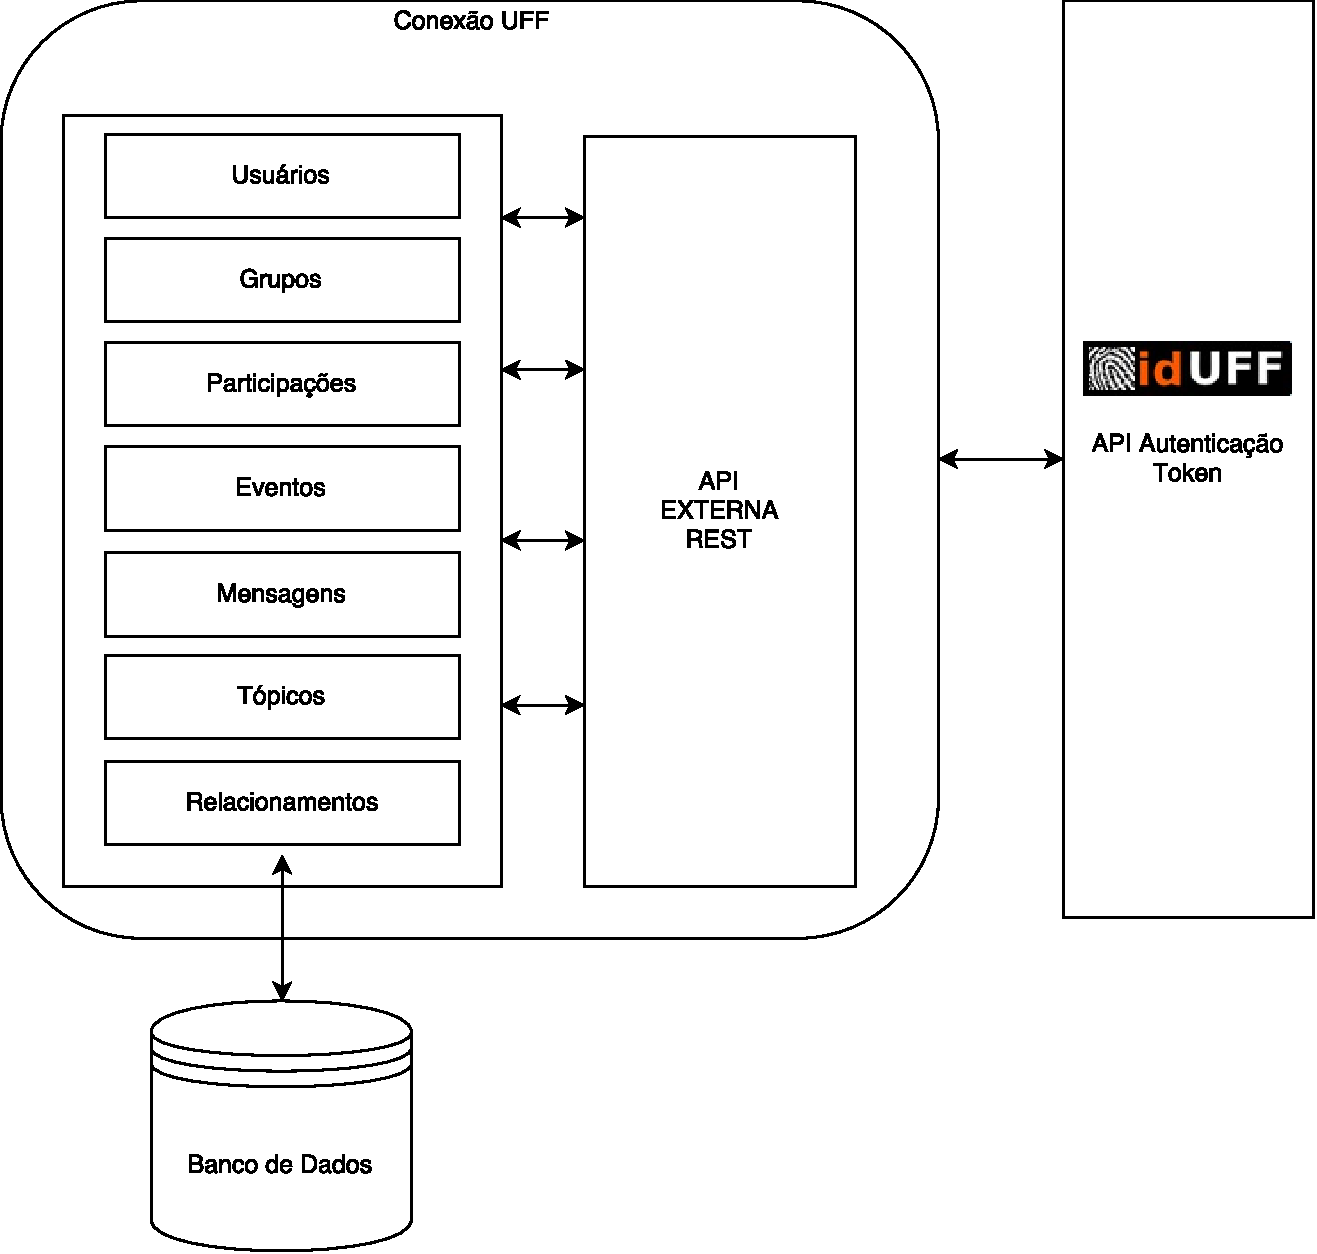
\includegraphics[scale=.65]{2_2.pdf}
    \caption{Arquitetura da camada de Serviços Conexão UFF}
    \label{conexao-arq}%
\end{figure}




\subsection{Moodle}

A plataforma mais utilizada para cursos acadêmicos on-line é o Moodle. O Moodle é um pacote de software especialmente concebido para ajudar professores a criar cursos online e oferece as funcionalidades de um LMS completo \cite{article:desnica-letic}

 O Moodle é um software de código aberto, que pode ser baixado gratuitamente a partir da Internet, usado, modificado, e até mesmo distribuído (sob uma licença GNU). O Moodle é facilmente executado em UNIX, Linux, Windows, Mac OS X, ou qualquer outro sistema que suporte PHP. Todos os seus dados são gravados em um único banco de dados, MySQL ou PostgreSQL são os mais suportados; no entanto, Oracle, Access, Interbase e ODBC  também podem ser utilizados com algumas configurações.
Dentre as funcionalidades do Moodle estão incluídos os fóruns, recursos de publicação de conteúdo, questionários, chats, atribuições, e outros recursos que geralmente são suficientes para a criação de cursos padrão. 

A unidade organizacional básica do Moodle é o curso, que é acessado através de uma página web. Um curso é organizado em seções que podem corresponder aos tópicos ou semanas, aparecendo na coluna do meio da página. É possível incluir diferentes recursos e atividades em todas as seções. O último está a ser atribuído como casa ou classe trabalho a ser desenvolvido pelos alunos. Os usuários são outro objeto Moodle essencial: eles podem se inscrever em cursos diferentes, como administradores, professores ou estudantes. Cada função é definida por suas capacidades em um determinado contexto, o que significa que eles têm um conjunto de privilégios ao executar determinadas ações \cite{article:isljamovic-petrovic}.

De acordo com o estudo realizado nos Estados Unidos \cite{article:wexler}, Blackboard e Moodle são os LMS com maior quota de mercado, sendo que o Moodle tem maior satisfação entre os usuários. Em nosso projeto, Blackboard foi descartado e escolhemos Moodle, pois além de ser \textit{Open Source}, ele já é utilizado em diversos cursos da \textit{UFF}.

\subsubsection{Camada de Serviços}
Moodle é composto por três elementos principais: o \textit{Core}, os módulos de atividades e os \textit{Plugins}. O \textit{Core} inclui as funcionalidades básicas da plataforma de aprendizagem, tais como o fórum, wiki e atividades.

Os \textit{Plugins} são blocos de software que adicionam extensões funcionais ao sistema. Dentro do Moodle, diferentes interfaces de plug-ins podem ser encontradas. Uma destas interfaces é a interface de Serviços Web, que é extensível e garante a escalabilidade do sistema em função dos diversos protocolos de comunicação.

Em 2008 foi projetada uma solução para fornecer algumas das funcionalidades através de Serviços Web, esta solução foi a Arquitetura de Serviços do Moodle, que foi implementada para Moodle 2.0 e lançada no final de 2009 \cite{article:alier}. 

A arquitetura de Serviços do Moodle acrescenta duas camadas lógicas à arquitetura do Moodle (mostrado na Figura \ref{moodle-arq}). A primeira é API externa, um conjunto de arquivos php que incluem a lógica de cada serviço. A segunda é a camada de conectores. A arquitetura de Serviços do Moodle não está vinculada a um protocolo de webservices específica; ele é projetada para ser independente de protocolo. Para cada protocolo suportado (SOAP, REST, XML-RPC, etc.) há um módulo conector específico nesta camada. Cada conector implementa a tradução dos métodos implementados na API externa com o protocolo e sintaxe específica. Além disso, o conector também oferece outros serviços necessários como autenticação, autorização e outros serviços de infra-estrutura. A camada de conectores é uma camada expansível que permite que o adição de novos protocolos de comunicação.

Um elemento-chave na concepção da arquitetura de Serviços do Moodle é sua capacidade de ampliação baseada em plugins. A API externa pode ser estendida de forma segura, dando total controle e segurança para o administrador da plataforma. Se for necessário um novo tipo de protocolo de serviços web ou método de autenticação, um desenvolvedor pode criar um novo conector de webservices para implementá-lo.

\begin{figure}[H]
\centering
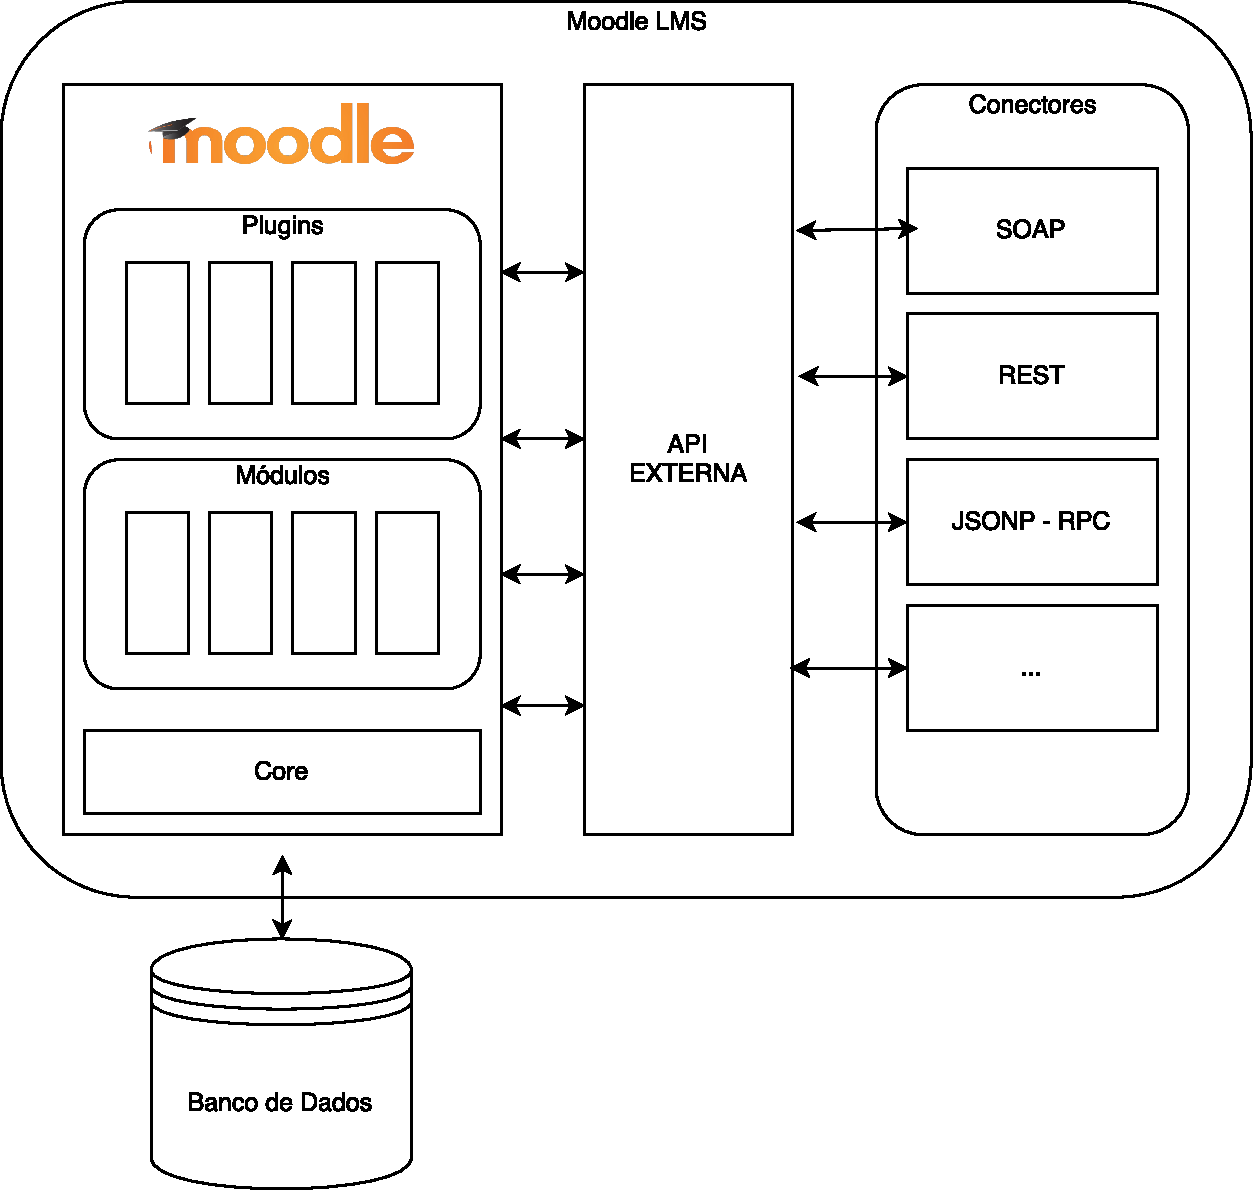
\includegraphics[scale=.65]{2_1.pdf}
    \caption{Arquitetura da camada de Serviços Moodle \cite{article:alier}}
    \label{moodle-arq}%
\end{figure}




\chapter{Especifica��o de Software}
\thispagestyle{empty} % retira numeracao da pagina, conforme as normas de apresentacao.

\section{Descri��o Geral}

\subsection{Perspectiva do produto}

O produto implementa uma interface para outros sistemas j� existentes estendendo suas funcionalidades. O produto consiste de uma aplica��o m�vel cliente e uma aplica��o web remota que acessa as interfaces p�blicas dos sistemas terceiros. A aplica��o web oferece uma API que atende os pedidos da aplica��o m�vel, intermediando o acesso aos sistemas externos.
A aplica��o web contar� com uma base de dados auxiliara, para controle dos usu�rios e comunica��o instant�nea.

\subsection{Fun��es do Produto}

O produto oferece como principais funcionalidades , T�picos (Grupo de Discuss�o), Envio de Arquivos, Calend�rio de Eventos da Disciplina, Mensageiro Instant�neo, Lista de Amigos e Envio de Mensagens.

\subsection{Classes de Usu�rio e Caracter�siticas}

As classes de usu�rios previstas ser�o, o aluno participante da disciplina, o professor da disciplina no papel de moderador do grupo, e os administradores do sistema que exercer�o fun��es de manuten��o do sistema.

\subsection{Ambiente Operacional}

A interface do usu�rio ser� executada em dispositivos m�veis como smartphones e tablets, nos tr�s sistemas operacionais mais utilizados, sendo eles o iOS da fabricante Apple, o Android da Google e o Windows Phone 8 da Microsoft.
A aplica��o remota ser� executada em uma m�quina servidora com sistema operacional Linux, distribui��o Ubuntu, com servidor web Apache ou Nginx com o m�dulo passenger-phusion devidamente configurado para servir aplica��es Ruby on Rails, todos em suas vers�es mais recentes.

\subsection{Restri��es de Design e Implementa��o}
Por se tratar de um trabalho acad�mico,  n�o haver�o restri��es de design e implementa��o r�gidas, deixando os desenvolvedores juntamente ao orientador livres para escolher as tecnologias verificadas e tidas como adequadas para a solu��o.

\subsection{Suposi��es e Depend�ncias}

O sistema tem como depend�ncias a plataforma de desenvolvimento m�vel Apache Cordova, o framework de desenvolvimento �gil Rails, o framework AngularJS, o framework de CSS Twitter Bootstrap e outros plugins ainda a serem indentificados no decorrer do desenvolvimento.

\section{Requisitos de Interface Externa}

\subsection{Interfaces de Usu�rio}
As interfaces de usu�rio ser�o desenvolvidas com as tecnologias e padr�es abertos web, Javascript, CSS3 e HTML5 e ser�o responsivas, se ajustando a diversos tipos de dispositivos e tamanhos de tela. Os esbo�os das interfaces s�o confeccionados com a ferramenta Ninja Mock e descrevem as principais interfaces no ap�ndice C.

\subsection{Interfaces de Hardware}

O software ser� executado em dispositivos m�veis, smartphones e tablets, do tipo Android, Windows e iPhone que se comunicar� com os servi�os de uma aplica��o intermedi�ria, executada em um computador servidor web, que por sua vez se comunica com as APIs das diversas plataformas de ensino.

\subsection{Interfaces de Software}

O software executado no dispositivo m�vel, utiliza o empasulamento de uma aplica��o web para as diversas plataformas m�veis atrav�s do framework phonegap, de forma totalmente transparente ao usu�rio que utiliza o software como um aplicativo nativo. Esta webapp se comunica com a aplica��o servidora intermedi�ria atrav�s de recursos web executados no software Apache ou Ngnx com o framework Rails. A aplica��o intermedi�ria por sua vez utiliza as intefaces disponibilizadas pelas plataformas de ensino, que podem ser diversas e implementadas sob a forma de plugins.

\subsection{Interfaces de Comunica��o}

A comunica��o � totalmente web, utilizando o protocolo HTTP entre a aplica��o cliente, a aplica��o web e as APIs das plataformas e ensino, seguindo o estilo arqutetural REST entre a a aplica��o cliente e a camada intermedi�ria.


\chapter{Integra UFF - Especificação de Requisitos do Software}
\thispagestyle{empty} % retira numeracao da pagina, conforme as normas de apresentacao.

Este capítulo apresenta a especificação de software do Integra UFF. Aqui serão descritos os objetivos, ambientes, suposições, requisitos e interfaces pensadas durante o desenvolvimento da mesma. Assim como as funcionalidades e telas implementadas no produto final. 

\section{Descrição Geral}

\subsection{Perspectiva do produto}

O produto implementa uma interface que agrega conteúdos obtidos de outros sistemas LMSs já existentes estendendo suas funcionalidades. Ele consiste de uma aplicação móvel cliente e uma aplicação web remota que acessa as interfaces públicas dos sistemas terceiros. A aplicação web oferece uma \textit{Application programming interface} (API) que atende os pedidos da aplicação móvel, intermediando o acesso aos sistemas externos.
A aplicação web contará com uma base de dados auxiliar, para controle dos usuários e comunicação instantânea.

\subsection{Funções do Produto}

A aplicação deve ser capaz permitir a autenticação do usuário nos sistemas integrados, obtendo o conteúdo necessário para fornecer as principais funcionalidades contempladas para o Integra UFF, que são:

\begin{itemize}
    \item Disponibilização de uma listagem das disciplinas do usuário.
    \item Tópicos (Grupo de Discussão).
    \item Listagem e \textit{download} de Arquivos.
    \item Calendário de Eventos das Disciplinas.
    \item Envio de Mensagens.
    \item Lista de Amigos.
\end{itemize}

\subsection{Classes de Usuário e Caracterísiticas}

As classes de usuários previstas serão, o aluno participante da disciplina, o professor da disciplina no papel de moderador do grupo, e os administradores do sistema que exercerão funções de manutenção do sistema. 

\subsection{Ambiente Operacional}

A interface do usuário será executada em dispositivos móveis como \textit{smartphones} e \textit{tablets}, nos três sistemas operacionais mais utilizados, sendo eles o iOS da fabricante \textit{Apple}, o \textit{Android} da \textit{Google} e o \textit{Windows Phone} 8 da \textit{Microsoft}.
A aplicação remota será executada em uma máquina servidora com sistema operacional Linux, distribuição Ubuntu, com servidor \textit{web} Apache ou Nginx com o módulo \textit{passenger-phusion} devidamente configurado para servir aplicações \textit{Ruby on Rails}, todos em suas versões mais recentes.

\subsection{Restrições de \textit{Design} e Implementação}
Por se tratar de um trabalho acadêmico,  não haverão restrições de \textit{design} e implementação rígidas, deixando os desenvolvedores juntamente ao orientador livres para escolher as tecnologias verificadas e tidas como adequadas para a solução. No entanto toda a integração feita com os sistemas LMSs são limitadas a disponibilidade de uma API acessível pela \textit{web} e ao conteúdo fornecido por elas. 

\subsection{Suposições e Dependências}

O sistema tem como dependências a plataforma de desenvolvimento móvel \textit{Apache Cordova}, o \textit{framework} de desenvolvimento ágil \textit{Rails}, o \textit{framework} AngularJS, o \textit{framework} de CSS \textit{Twitter Bootstrap} e outros \textit{plugins} indentificados no decorrer do desenvolvimento.

\section{Requisitos de Interface Externa}

\subsection{Interfaces de Usuário}
As interfaces de usuário serão desenvolvidas com as tecnologias e padrões abertos \textit{web}, \textit{Javascript}, CSS3 e HTML5 e serão responsivas, se ajustando a diversos tipos de dispositivos e tamanhos de tela.

\subsection{Interfaces de Hardware}

O \textit{software} será executado em dispositivos móveis, \textit{smartphones} e \textit{tablets}, do tipo \textit{Android}, \textit{Windows} e \textit{iPhone} que se comunicará com os serviços de uma aplicação intermediária, executada em um computador servidor \textit{web}, que por sua vez se comunica com as APIs das diversas plataformas de ensino integradas.

\subsection{Interfaces de Software}

O \textit{software} executado no dispositivo móvel, utiliza o empasulamento de uma aplicação \textit{web} para as diversas plataformas móveis através do \textit{framework} \textit{phonegap}, de forma totalmente transparente ao usuário que utiliza o \textit{software} como um aplicativo nativo. Esta \textit{webapp} se comunica com a aplicação servidora intermediária através de recursos \textit{web} executados no \textit{software} Apache ou \textit{Ngnx} com o \textit{framework} \textit{Rails}. A aplicação intermediária por sua vez utiliza as intefaces disponibilizadas pelas plataformas de ensino, que podem ser diversas e implementadas sob a forma de \textit{plugins}.

\subsection{Interfaces de Comunicação}

A comunicação é totalmente via \textit{web}, utilizando o protocolo HTTP entre a aplicação cliente, a aplicação servidor e as APIs das plataformas de ensino, seguindo o estilo arqutetural REST entre a a aplicação cliente e a camada intermediária.

\section{Funcionalidades do Sistema}

Nesta seção descreveremos as funcionalidades implementadas na versão final do aplicativo Integra UFF, assim como suas telas.

\subsection{Sincronizar com uma plataforma}

O primeiro passo para começar a utilizar o Integra UFF é realizar a sincronização com uma das plataformas integradas. Atualmente apenas o Conexão UFF está disponível. 

Ao acessar o aplicativo o usuário verá uma tela com um botão de sincronização, que ao apertado exibirá um formulário de autenticação, figura \ref{sincronizacao}. Feito a autenticação, o usuário será redirecionado para o menu principal do aplicativo, figura \ref{menuprincipal}, com o acesso a Disciplinas, Eventos e Arquivos. 

O caso de uso da sincronização está explicitado na tabela \ref{table:sincronizacao}.

\begin{figure}[H]
    \centering
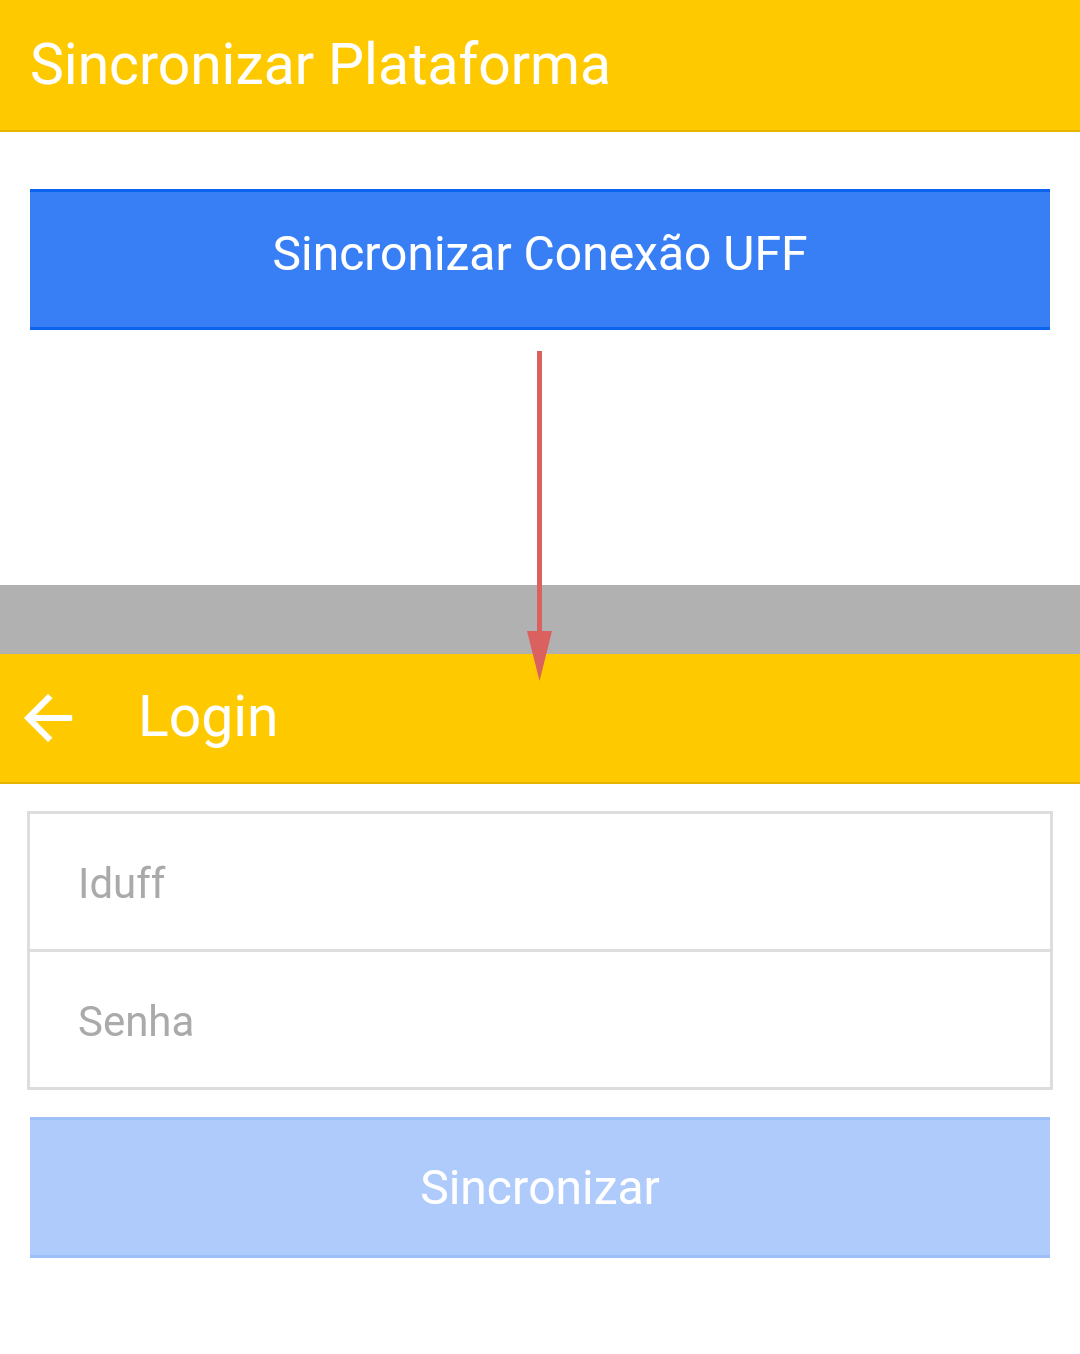
\includegraphics[scale=0.15]{sincronizacao}
    \caption{Autenticação na plataforma}
    \label{sincronizacao}
\end{figure}

\begin{figure}[H]
    \centering
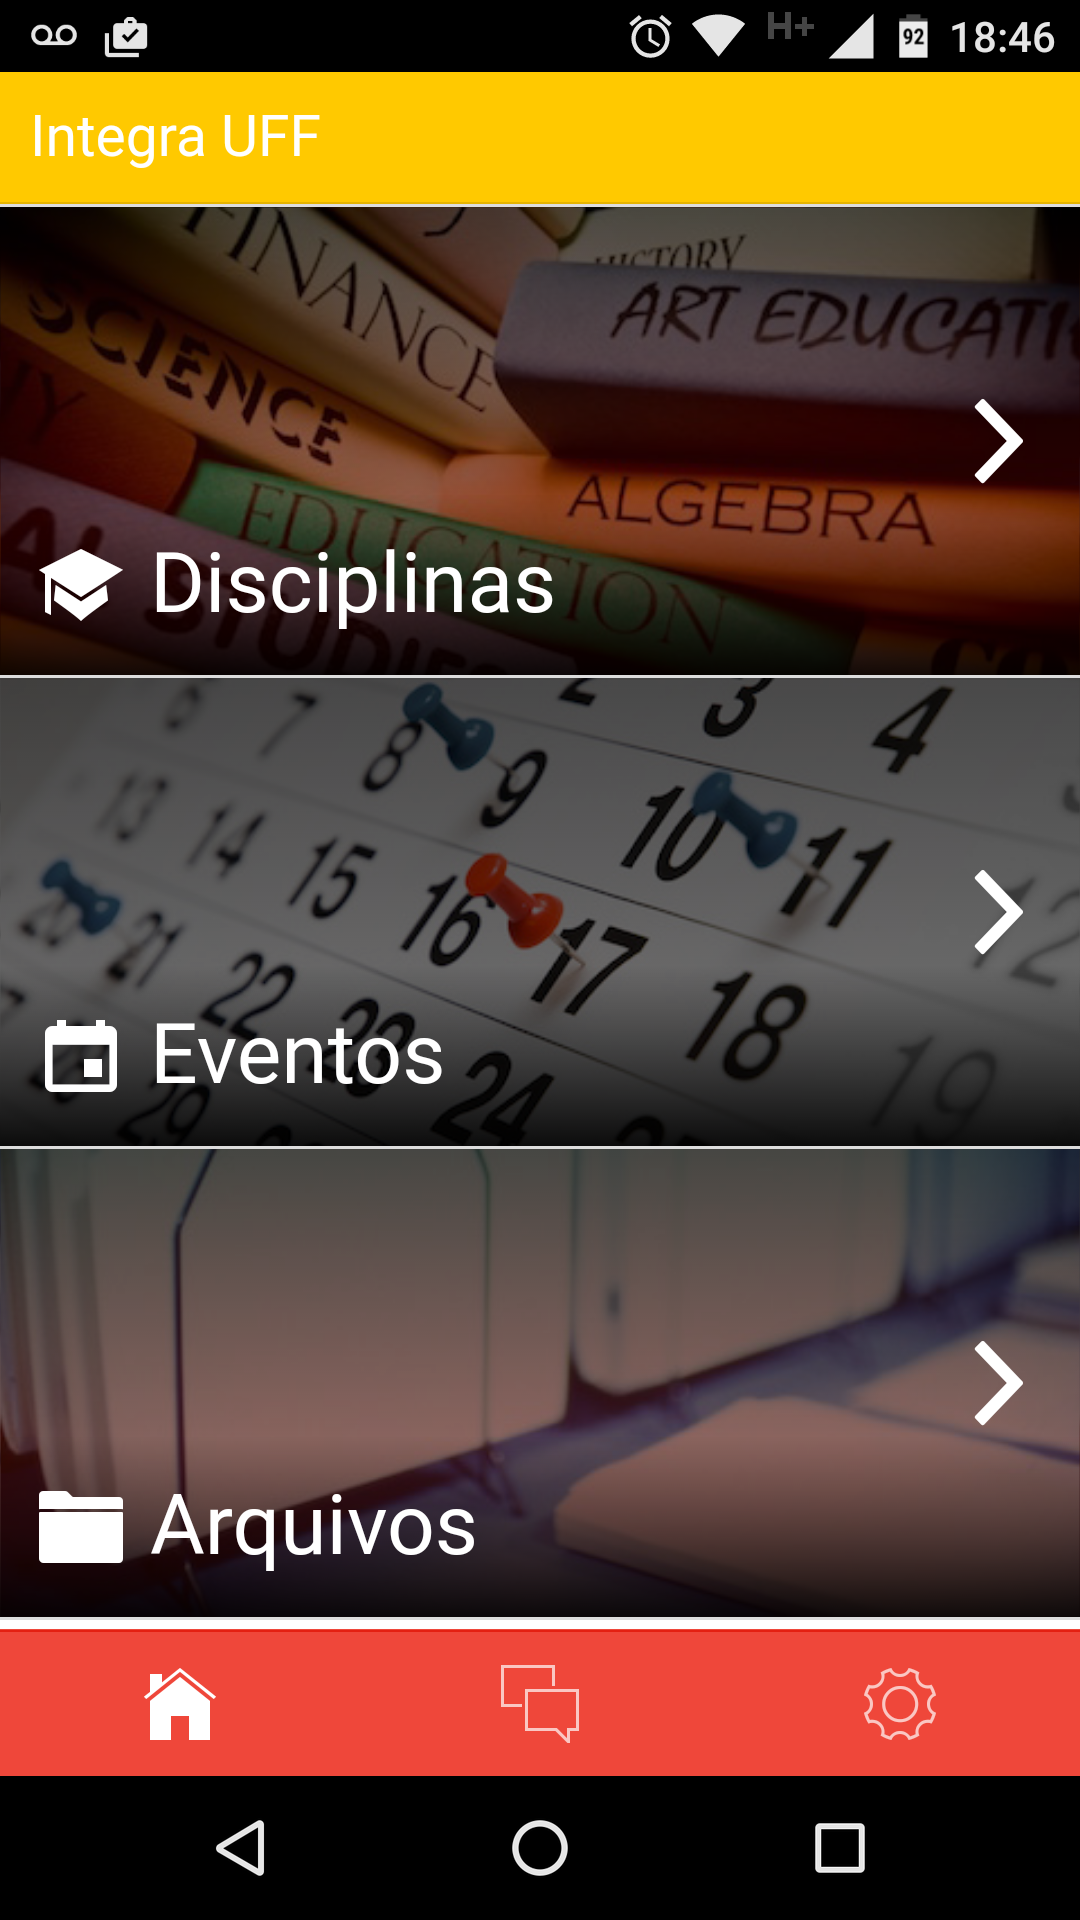
\includegraphics[scale=0.15]{menuprincipal}
    \caption{Menu do Integra UFF}
    \label{menuprincipal}
\end{figure}

\begin{table}[H]
  \begin{tabular}{ p{.20\textwidth} | p{.80\textwidth} }
    Trigger & O usuário acessa a aplicação\\
    \hline
    Pré condição & O usuário não sincronizou com nenhuma das aplicações anteriormente. O aparelho deve estar conectado à internet.\\
    \hline
    Caminho Básico &
    \begin{minipage}{5in}
      \vskip 4pt
      \begin{enumerate}
        \item O usuário escolhe a qual rede deseja se conectar selecionando com o toque na tela em um item dentre uma lista de opções.
        \item O sistema exibe um formulário de login com um campo para o e-mail e outro para a senha.
        \item O usuário preenche seus dados e seleciona sincronizar.
        \item O sistema sincroniza com a aplicação escolhida e exibe a tela principal com as opções Disciplinas, Eventos, Arquivos e Configurações.
      \end{enumerate}
      \vskip 4pt
    \end{minipage} \\
    \hline
    Caminho alternativo &
    \begin{minipage}{5in}
      \vskip 4pt
      Se o usuário já sincronizou com alguma aplicação anteriormente ele deve seguir os seguintes passos:
      \begin{enumerate}
        \item O usuário seleciona Configurações na tela principal.
        \item O usuário seleciona Contas Sincronizadas na tela de configurações.
        \item O sistema exibe a tela com as opções de aplicações disponíveis para sincronização.
        \item A partir daqui o usuário segue o caminho básico.
      \end{enumerate}
      \vskip 4pt
    \end{minipage} \\
    \hline
    Pós condição & Informações da aplicação sincronizada devem ser baixadas para o aparelho.\\
    \hline
    Caminho de exceção & O usuário pode abandonar a operação a qualquer momento. Caso o usuário erre o login o sistema deve exibir a tela de login informando o erro.
  \end{tabular}
  \caption{Sincronizar com uma aplicação}
  \label{table:sincronizacao}
\end{table}

\subsection{Acessar listagem de disciplinas}

As disciplinas representam o conteúdo principal da aplicação. Todos os outros conteúdos estão associados a ela. Portanto se fez necessário exibir uma listagem delas para o usuário, a qual é acessada pelo menu principal demonstrado anteriormente.

A listagem possui uma interface simples que informa o nome das disciplinas associadas e o semestre a qual ela pertence como mostra a figura \ref{indexdisciplinas}.

\begin{figure}[H]
    \centering
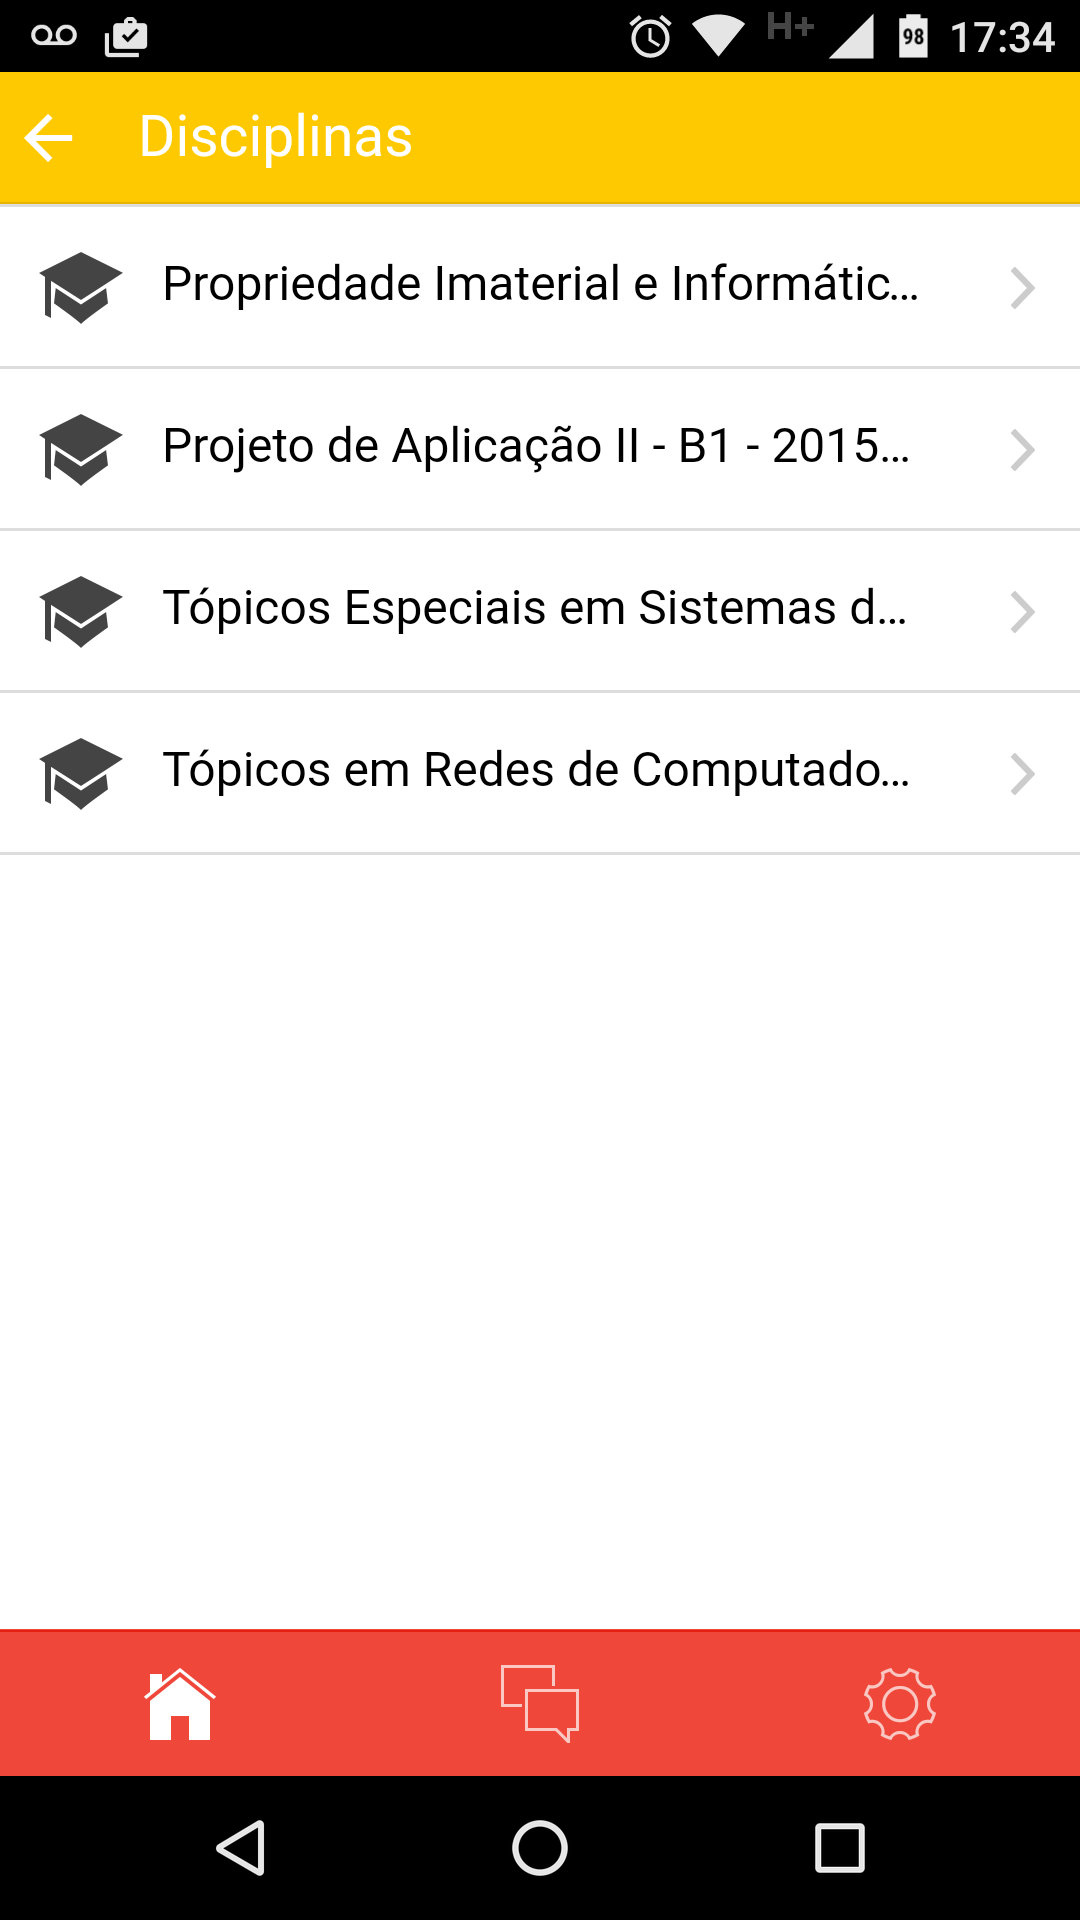
\includegraphics[scale=0.15]{indexdisciplinas}
    \caption{Listagem de Disciplinas}
    \label{indexdisciplinas}
\end{figure}

Ao clicar no nome de uma das disciplinas da lista, o usuário será redirecionado para uma seção contendo os detalhes da mesma.

O caso de uso desta funcionalidade é mostrado na tabela \ref{table:indexdisciplinas}.

\begin{table}[H]

  \begin{tabular}{ p{.20\textwidth} | p{.80\textwidth} }
    Trigger & O usuário acessa a aplicação.\\
    \hline
    Pré condição & O usuário está na tela do menu principal do sistema.\\
    \hline
    Caminho Básico &
    \begin{minipage}{5in}
      \vskip 4pt
      \begin{enumerate}
        \item O usuário seleciona a opção disciplinas no menu do sistema.
        \item O sistema exibe uma tela com uma lista de todas as disciplinas sincronizadas com o aparelho. A listagem contém o nome da disciplina.
      \end{enumerate}
      \vskip 4pt
    \end{minipage} \\
    \hline
    Caminho de exceção & O usuário pode abandonar a operação a qualquer momento.
 \end{tabular}
 \caption{Acessar listagem de disciplinas}
 \label{table:indexdisciplinas}
\end{table}

\subsection{Acessar detalhes de disciplinas}

Os detalhes de cada disciplina podem ser acessados através do clique em seu nome exibido na listagem. Nesta tela serão exibidas uma lista de tópicos, eventos e arquivos associados àquela disciplina, conforme a figura \ref{showdisciplina}, viabilizando uma forma simples de visualizar todos os conteúdos de uma disciplina específica.

\begin{figure}[H]
    \centering
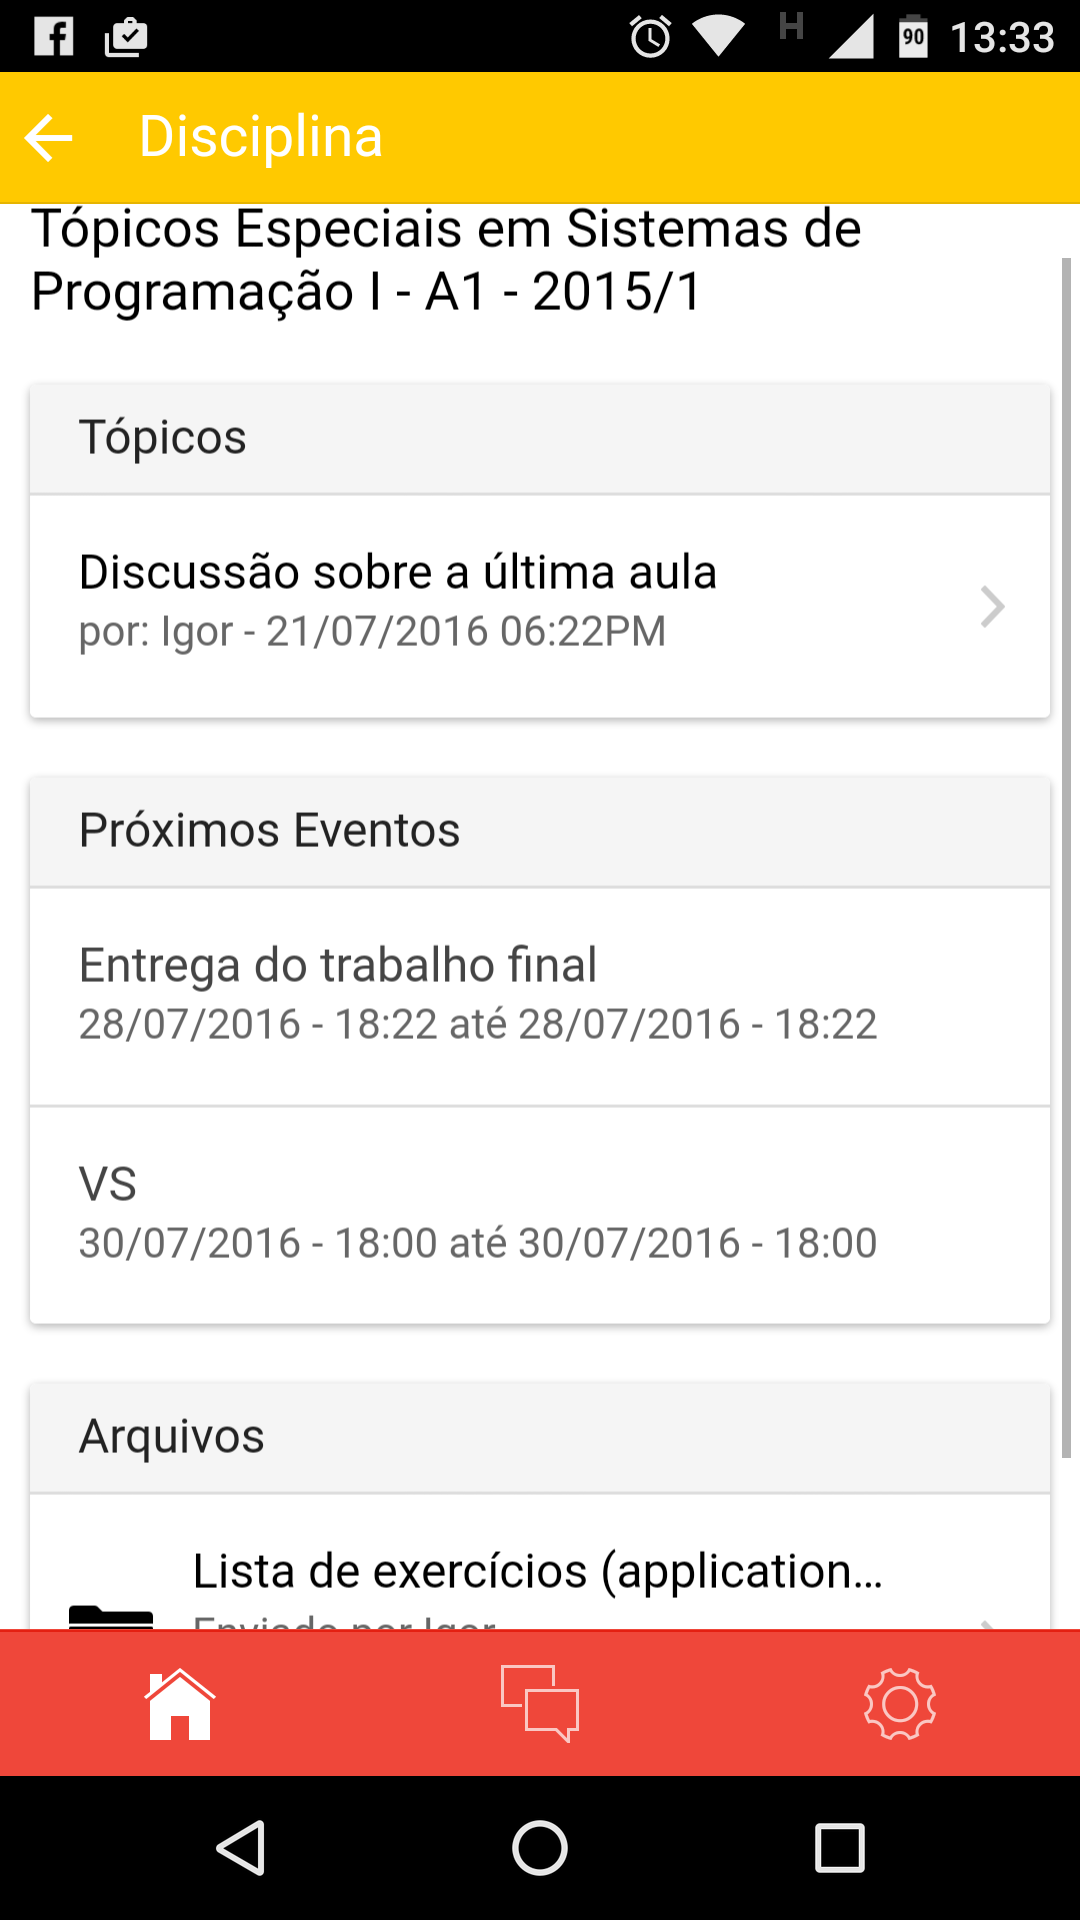
\includegraphics[scale=0.15]{showdisciplina}
    \caption{Detalhes de uma Disciplina}
    \label{showdisciplina}
\end{figure}

O clique no nome de um arquivo ou tópico redireciona o usuário para a página de detalhes dos mesmos.

O caso de uso desta funcionalidade é mostrado na tabela \ref{table:showdisciplina}.

\begin{table}[H]
  \begin{tabular}{ p{.20\textwidth} | p{.80\textwidth} }
    Trigger & O usuário acessou a tela de listagem de disciplinas.\\
    \hline
    Pré condição & O usuário possui alguma disciplina sincronizada com o aparelho.\\
    \hline
    Caminho Básico &
    \begin{minipage}{5in}
      \vskip 4pt
      \begin{enumerate}
        \item O usuário seleciona uma das disciplinas da listagem.
        \item O sitema exibe uma tela contendo as seguintes informações sobre a disciplina: nome, últimos tópicos, próximos eventos e últimos arquivos.
      \end{enumerate}
      \vskip 4pt
    \end{minipage} \\
    \hline
    Caminho de exceção & O usuário pode abandonar a operação a qualquer momento.
  \end{tabular}
  \caption{Acessar detalhes de disciplinas}
  \label{table:showdisciplina}
\end{table}

\subsection{Acessar listagem de arquivos}

Apesar de ser possível acessar a lista de arquivos de uma disciplina na tela de listagem da última, também está disponível uma listagem de arquivos sincronizados através do clique na opção Arquivos no menu principal da aplicação. Esta listagem demonstra todos os arquivos sicronizados, agrupados pelas disciplinas a qual pertencem, como mostra a figura \ref{indexarquivos}

\begin{figure}[H]
    \centering
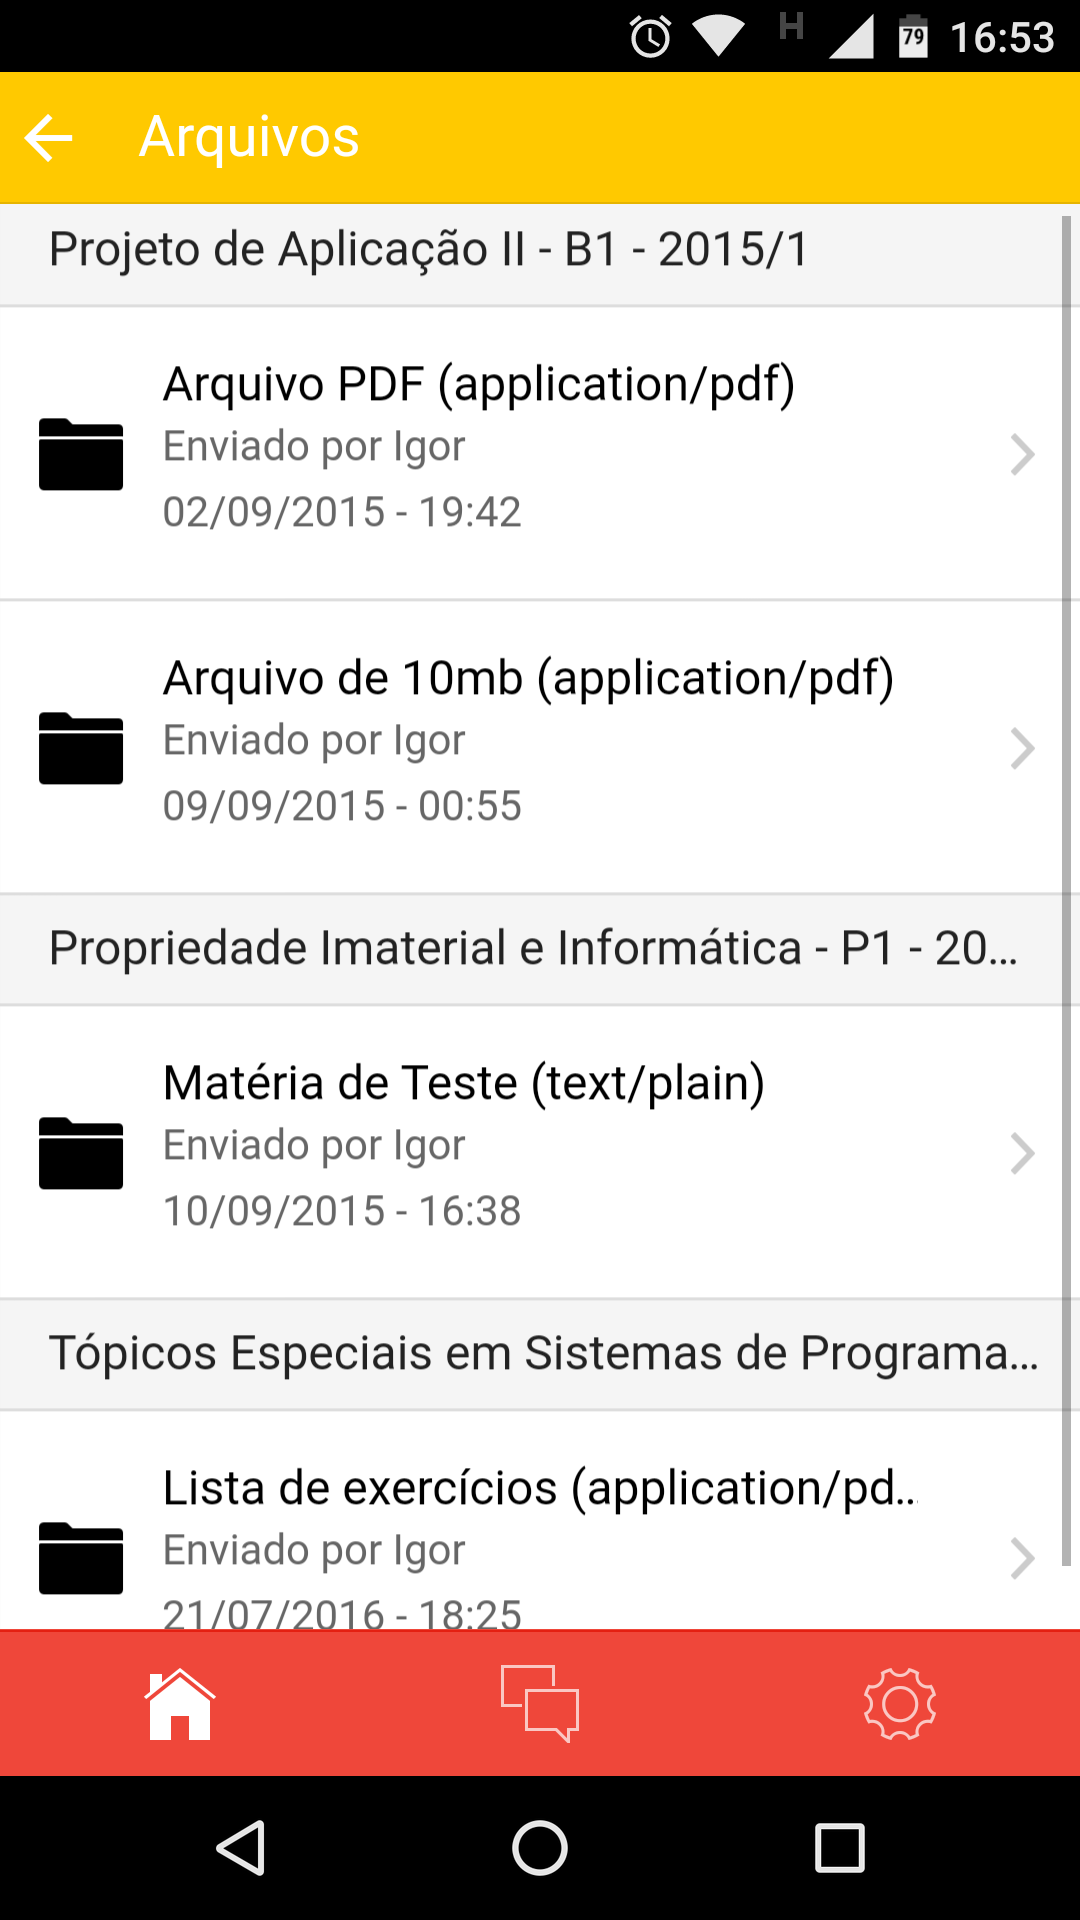
\includegraphics[scale=0.15]{indexarquivos}
    \caption{Listagem de Arquivos}
    \label{indexarquivos}
\end{figure}

Clicando em qualquer um dos arquivos o usuário será redirecionado para a página de detalhes deste. A tabela \ref{table:indexarquivos} apresenta o caso de uso desta funcionalidade.

\begin{table}[H]
  \begin{tabular}{ p{.20\textwidth} | p{.80\textwidth} }
    Trigger & O usuário acessa a aplicação.\\
    \hline
    Pré condição & O usuário possui alguma disciplina sincronizada com o aparelho.\\
    \hline
    Caminho Básico &
    \begin{minipage}{5in}
      \vskip 4pt
      \begin{enumerate}
        \item O usuário seleciona a opção arquivos no menu do sistema.
        \item O sistema exibe uma tela com uma lista de todos os arquivos sincronizados com o aparelho. A listagem contém as seguintes informações dos arquivos: nome, formato, quem o enviou, data e hora de envio. Os arquivos exibidos são organizados por disciplinas.
      \end{enumerate}
      \vskip 4pt
    \end{minipage} \\
    \hline
    Caminho de exceção & O usuário pode abandonar a operação a qualquer momento.
  \end{tabular}
  \caption{Acessar listagem de arquivos}
  \label{table:indexarquivos}
\end{table}

\subsection{Acessar detalhes de arquivos}

Conforme as citações anteriores a página de detalhes de arquivos pode ser acessada através da listagem geral de arquivos, ou da listagem de arquivos na tela de detalhes de uma disciplina. Esta tela contém o nome do arquivo e informações do formato, tamanho, data e hora em que foi enviado e o nome de quem o enviou, visto na figura \ref{showarquivo}. Além de possuir um botão para realizar o \textit{download} para o dispositivo.  

\begin{figure}[H]
    \centering
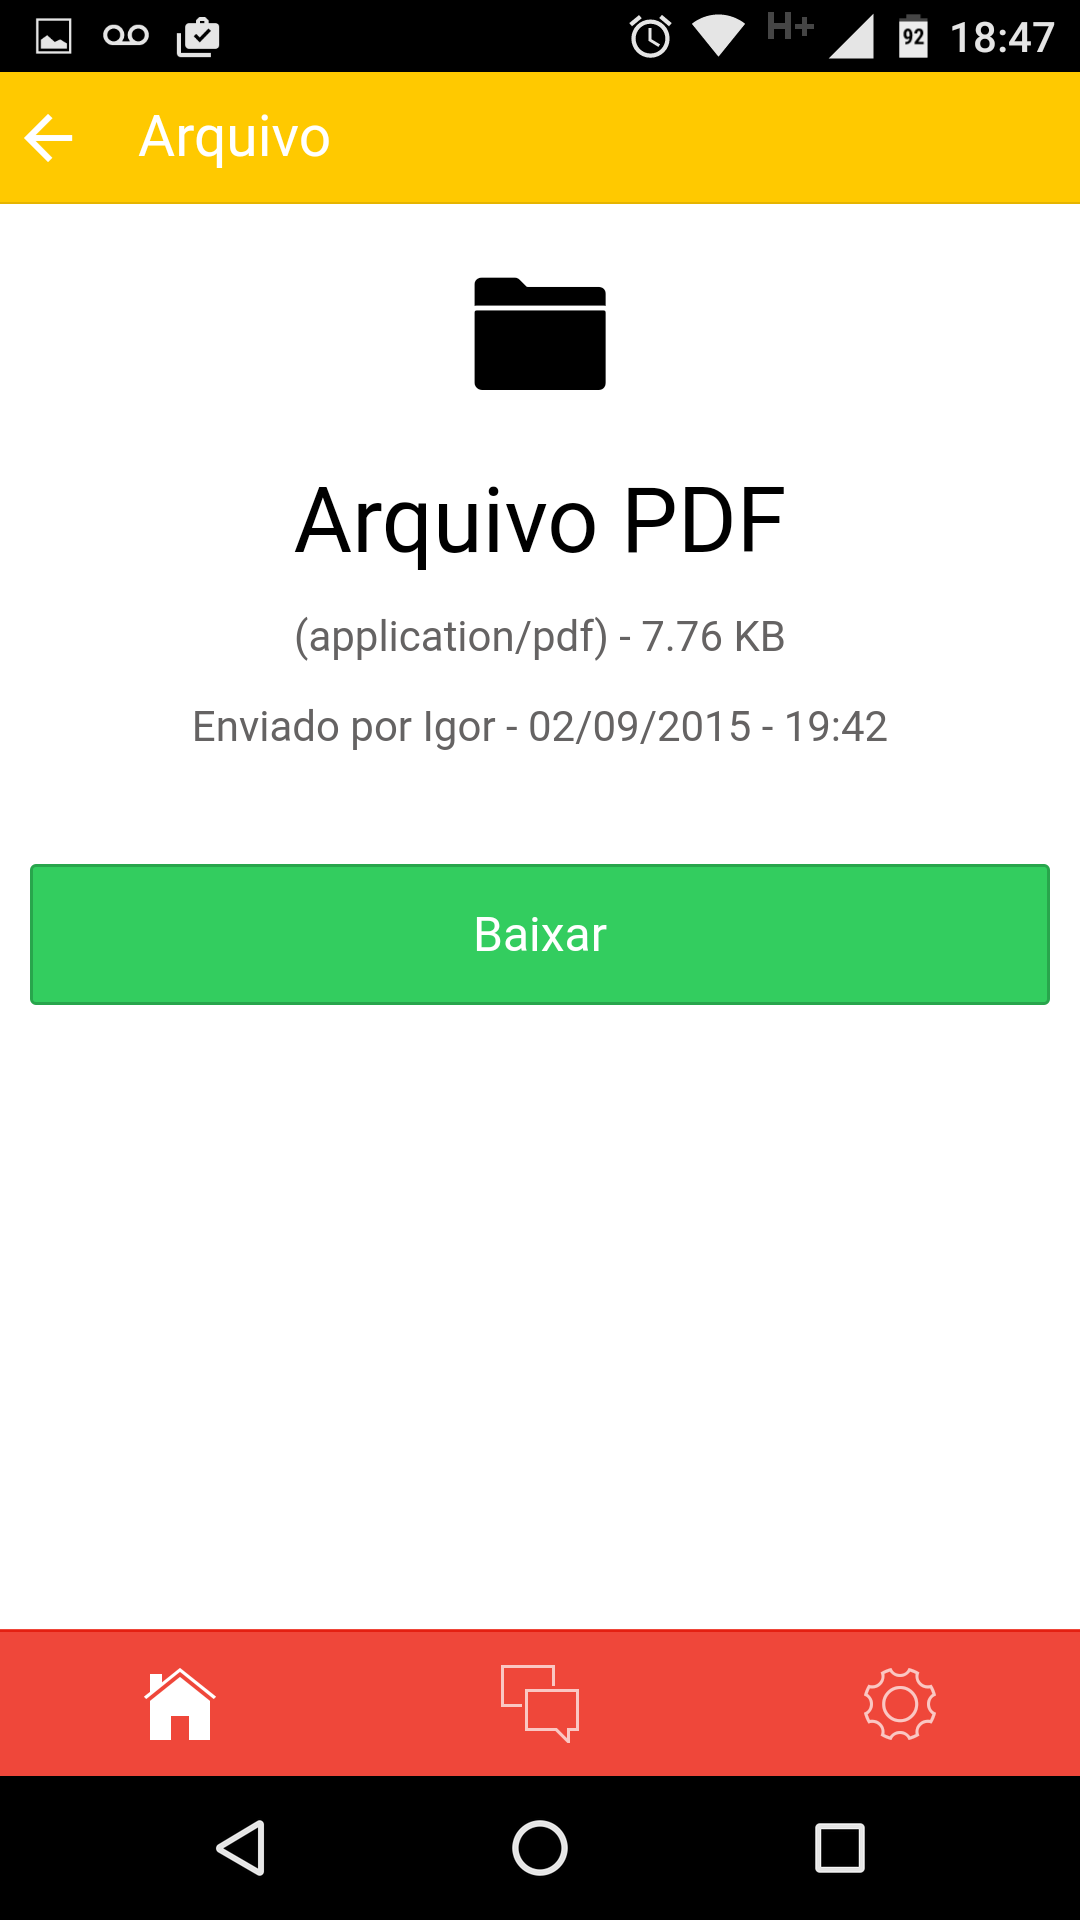
\includegraphics[scale=0.15]{showarquivo}
    \caption{Detalhes de um Arquivo}
    \label{showarquivo}
\end{figure}

Caso o arquivo já tenha sido baixado, a tela irá exibir um botão para abri-lo e um \textit{link} para apagá-lo.

A tabela \ref{table:showarquivo} evidencia o caso de uso.

\begin{table}[H]
  \begin{tabular}{ p{.20\textwidth} | p{.80\textwidth} }
    Trigger & O usuário acessou a tela de listagem de arquivos.\\
    \hline
    Pré condição & O usuário possui algum arquivo sincronizado com o aparelho.\\
    \hline
    Caminho Básico &
    \begin{minipage}{5in}
      \vskip 4pt
      \begin{enumerate}
        \item O usuário seleciona um dos arquivos da listagem.
        \item O sitema exibe uma tela contendo as seguintes informações sobre o arquivo: nome, formato, tamanho, quem o enviou, data e hora do envio, um botão para baixá-lo.
      \end{enumerate}
      \vskip 4pt
    \end{minipage} \\
    \hline
    Caminho de exceção & O usuário pode abandonar a operação a qualquer momento.
  \end{tabular}
  \caption{Acessar detalhes de arquivos}
  \label{table:showarquivo}
\end{table}

\subsection{Baixar arquivos}

Baixar os arquivos é possível através de um botão na tela de detalhes de um arquivo. O procedimento é demonstrado pela figura \ref{downloadarquivo} e o caso de uso pela tabela \ref{table:downloadarquivo}.

\begin{figure}[H]
    \centering
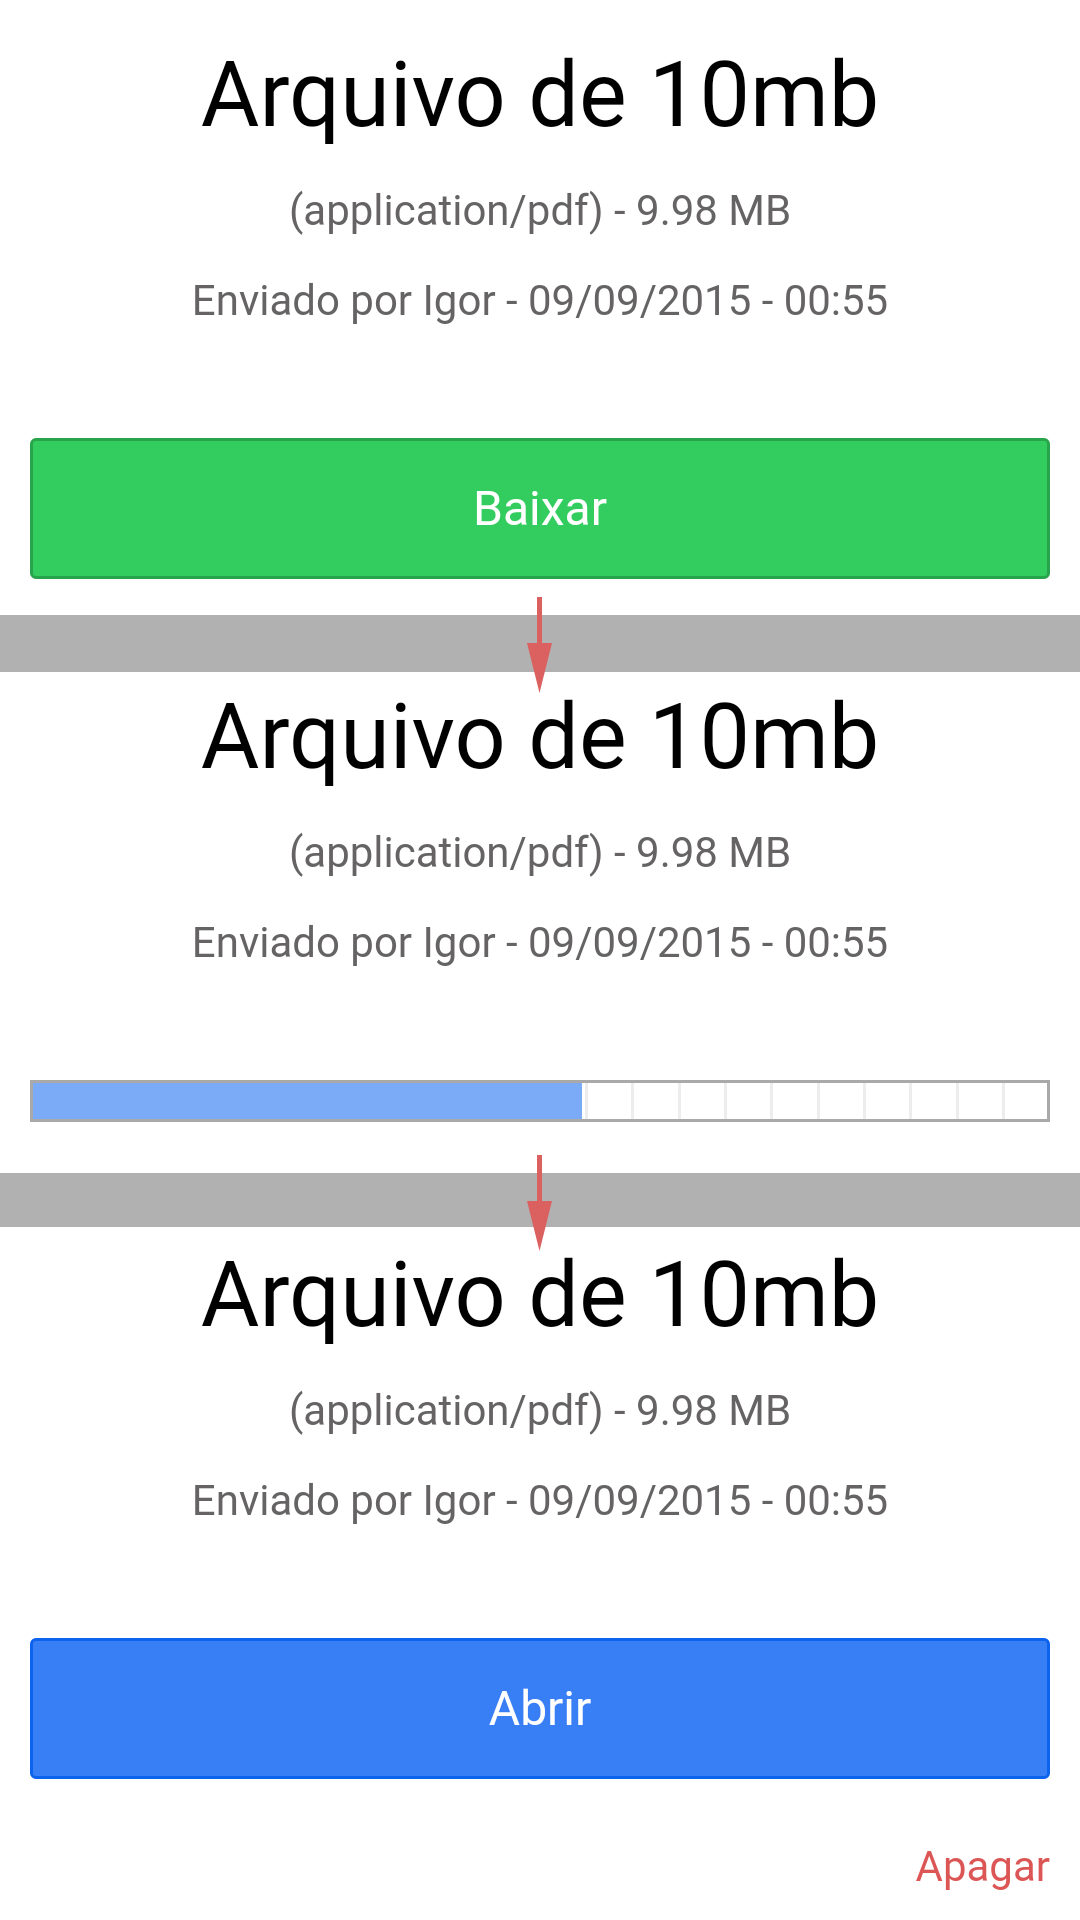
\includegraphics[scale=0.15]{downloadarquivo}
    \caption{\textit{Download} de um Arquivo}
    \label{downloadarquivo}
\end{figure}

\begin{table}[H]
  \begin{tabular}{ p{.20\textwidth} | p{.80\textwidth} }
    Trigger & O usuário acessa a página de detalhes de um arquivo.\\
    \hline
    Pré condição & O usuário possui algum arquivo sincronizado com o aparelho. O aparelho deve estar conectado à internet.\\
    \hline
    Caminho Básico &
    \begin{minipage}{5in}
      \vskip 4pt
      \begin{enumerate}
        \item O usuário aperta o botão download.
        \item O sistema inicia o download do arquivo selecionado.
      \end{enumerate}
      \vskip 4pt
    \end{minipage} \\
    \hline
    Pós condição & O arquivo selecionado deve ser baixado para o aparelho do usuário e o sistema deve mostrar os botões para abrir e apagar o arquivo.\\
    \hline
    Caminho de exceção & O usuário pode abandonar a operação a qualquer momento.\\
    \hline
  \end{tabular}
  \caption{Baixar arquivos}
  \label{table:downloadarquivo}
\end{table}

\subsection{Apagar arquivos}

Apagar os arquivos, assim como o seu \textit{download}, é realizado através de um \textit{link} na tela de detalhes de um arquivo. O procedimento é demonstrado pela figura \ref{apagararquivo} e o caso de uso pela tabela \ref{table:apagararquivo}.

\begin{figure}[H]
    \centering
\includegraphics[scale=0.15]{apagararquivo}
    \caption{Apagar um Arquivo}
    \label{apagararquivo}
\end{figure}


\begin{table}[H]
  \begin{tabular}{ p{.20\textwidth} | p{.80\textwidth} }
    Trigger & O usuário acessa a página de detalhes de um arquivo.\\
    \hline
    Pré condição & O usuário possui algum arquivo baixado no aparelho.\\
    \hline
    Caminho Básico &
    \begin{minipage}{5in}
      \vskip 4pt
      \begin{enumerate}
        \item O usuário aperta o botão apagar.
      \end{enumerate}
      \vskip 4pt
    \end{minipage} \\
    \hline
    Pós condição & O arquivo selecionado deve ser apagado do aparelho do usuário e o sistema deve exibir o botão para baixar o arquivo.\\
    \hline
    Caminho de exceção & O usuário pode abandonar a operação a qualquer momento.\\
    \hline
  \end{tabular}
  \caption{Apagar arquivos}
  \label{table:apagararquivo}
\end{table}

\subsection{Acessar listagem de eventos}

A listagem de eventos reúne todos os eventos sincronizados no dispositivo. Os eventos são agrupados por próximos, eventos prestes a acontecerem, e encerrados como mostra a figura \ref{indexeventos}. Esta listagem também informa a qual disciplina cada evento pertence.

\begin{figure}[H]
    \centering
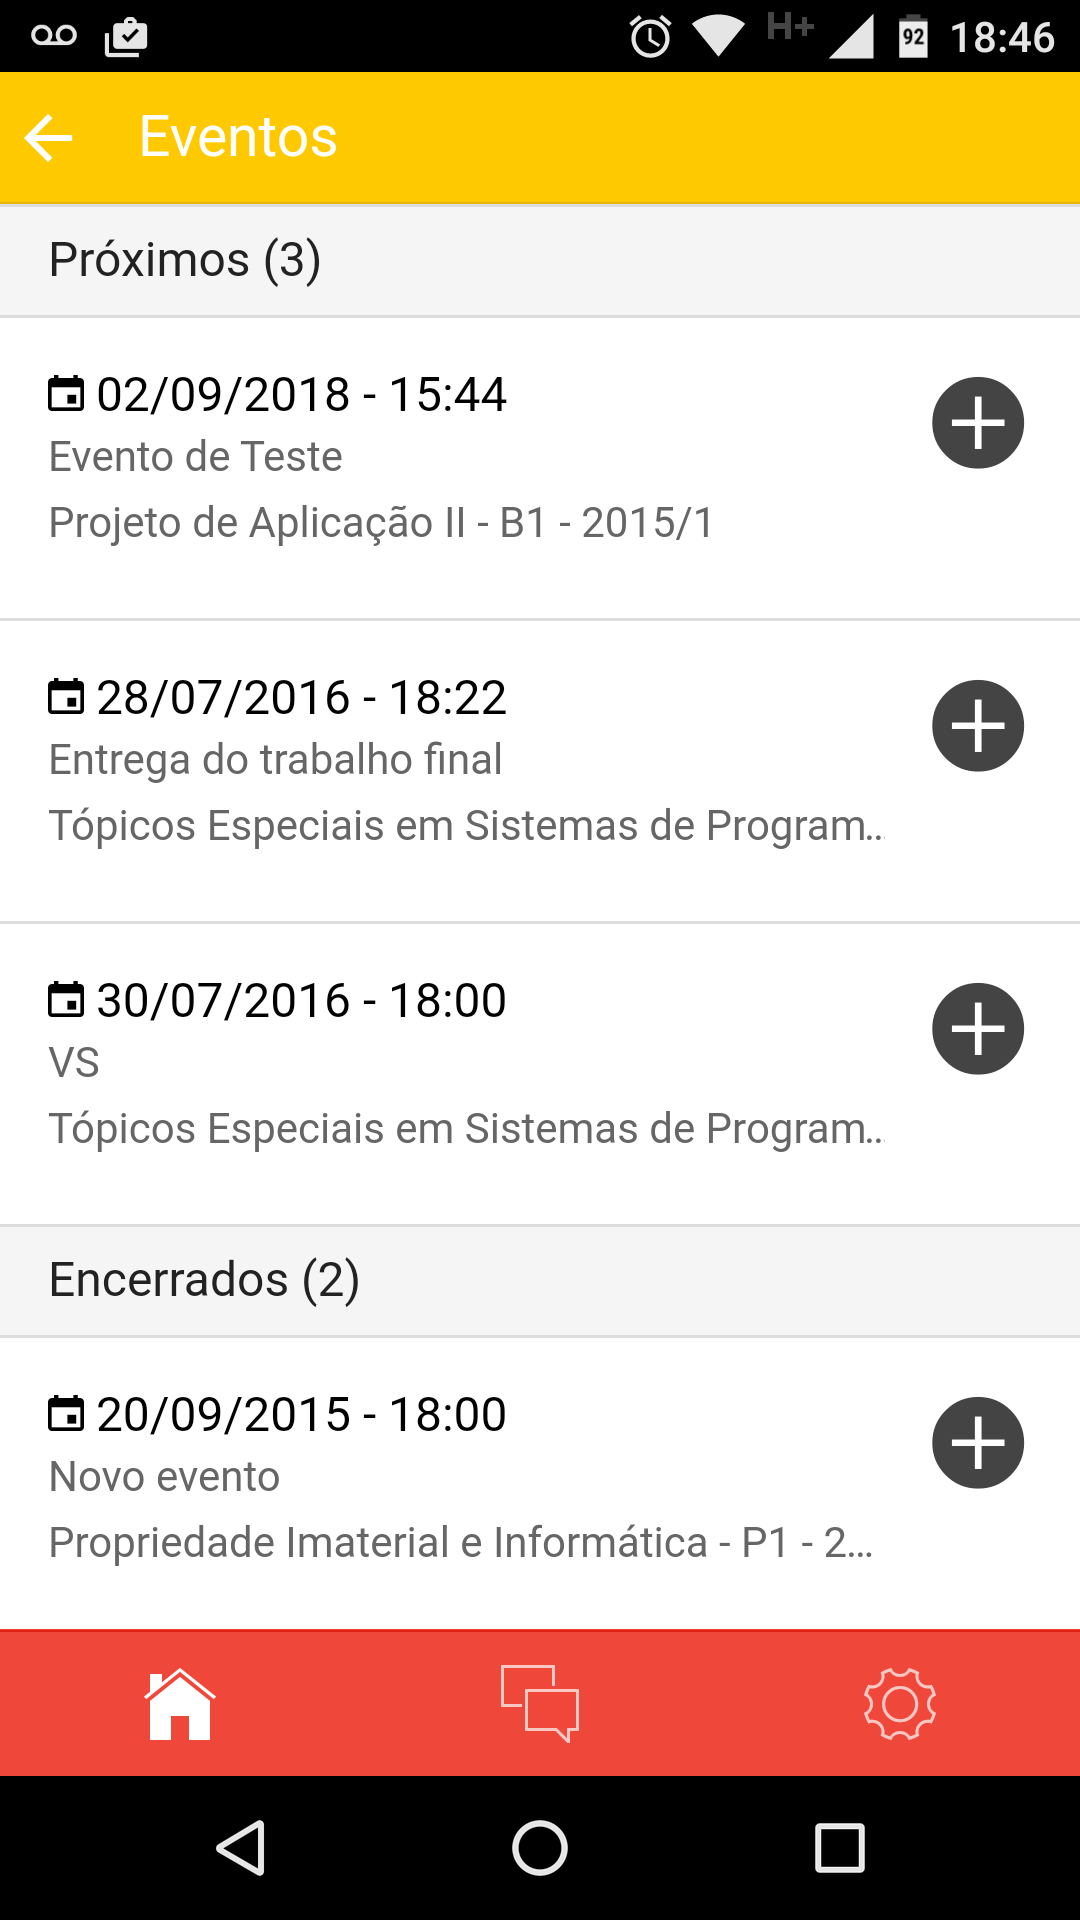
\includegraphics[scale=0.15]{indexeventos}
    \caption{Listagem de Eventos}
    \label{indexeventos}
\end{figure}

O caso de uso pode ser observado na tabela \ref{table:indexeventos}.

\begin{table}[H]
  \begin{tabular}{ p{.20\textwidth} | p{.80\textwidth} }
    Trigger & O usuário acessa a aplicação.\\
    \hline
    Pré condição & O usuário está na tela do menu principal do sistema.\\
    \hline
    Caminho Básico &
    \begin{minipage}{5in}
      \vskip 4pt
      \begin{enumerate}
        \item O usuário seleciona a opção eventos no menu do sistema.
        \item O sistema exibe uma tela com uma lista de todos os eventos sincronizados com o aparelho. A listagem contém as seguintes informações dos eventos: nome, data, hora e disciplina. Os eventos são exibidos separadamente entre próximos eventos e eventos passados.
      \end{enumerate}
      \vskip 4pt
    \end{minipage} \\
    \hline
    Caminho de exceção & O usuário pode abandonar a operação a qualquer momento.\\
    \hline
  \end{tabular}
  \caption{Acessar listagem de eventos}
  \label{table:indexeventos}
\end{table}

\subsection{Adicionar evento ao calendário}

Os eventos podem ser adicionados no calendário padrão do dispositivo utilizado pelo usuário. Para isso é preciso acessar a listagem dos eventos e clicar no ícone ao lado direito do evento escolhido. Uma caixa de diálogo será exibida confirmando a operação. A figura \ref{addevento} ilustra o procedimento, e o caso de uso é descrito pela tabela \ref{table:addevento}.

\begin{figure}[H]
    \centering
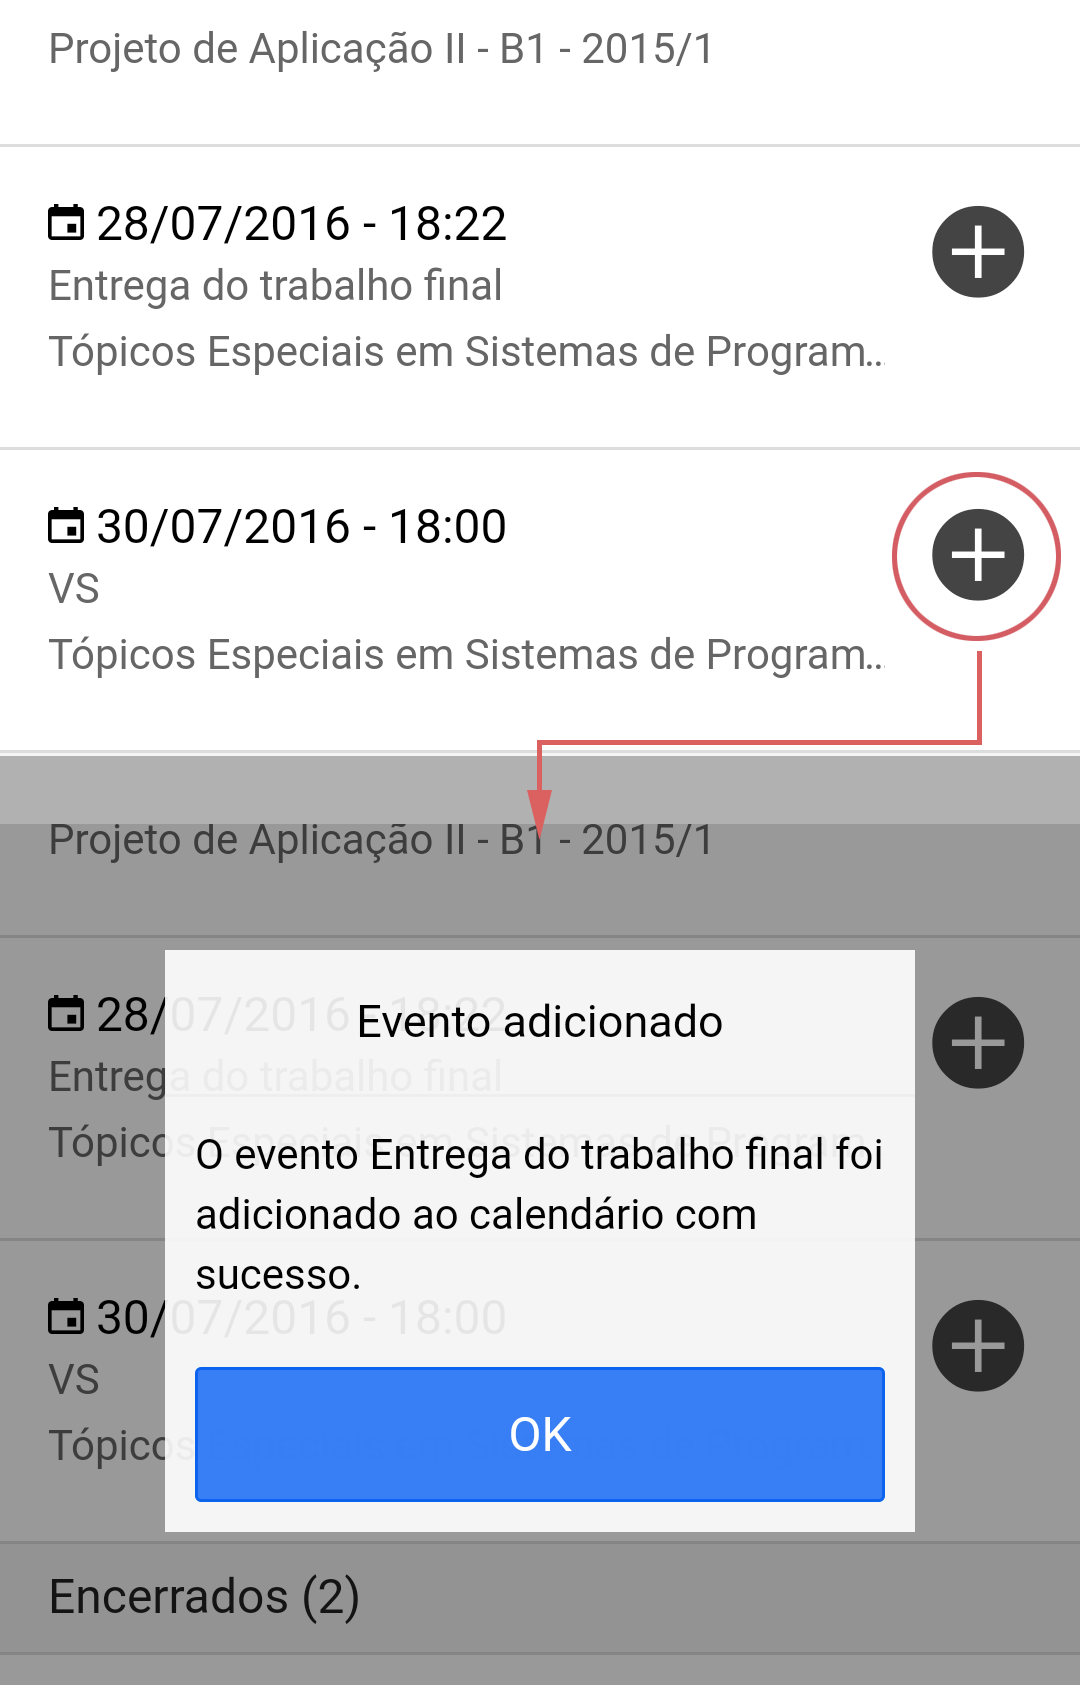
\includegraphics[scale=0.15]{addevento}
    \caption{Adicionar evento ao calendário}
    \label{addevento}
\end{figure}

\begin{table}[H]
  \begin{tabular}{ p{.20\textwidth} | p{.80\textwidth} }
    Trigger & O usuário acessa a página de listagem de eventos.\\
    \hline
    Pré condição & O usuário possui algum evento sincronizado no aparelho.\\
    \hline
    Caminho Básico &
    \begin{minipage}{5in}
      \vskip 4pt
      \begin{enumerate}
        \item O usuário seleciona o ícone de adicionar situado ao lado do evento que deseja colocar no calendário.
      \end{enumerate}
      \vskip 4pt
    \end{minipage} \\
    \hline
    Pós condição & O evento selecionado deve ser criado no calendário nativo do aparelho do usuário.\\
    \hline
    Caminho de exceção & O usuário pode abandonar a operação a qualquer momento.\\
    \hline
  \end{tabular}
  \caption{Adicionar evento ao calendário}
  \label{table:addevento}
\end{table}

\section{Outros requisitos não funcionais}

\subsection{Requisitos de segurança}

Para a utilização do sistema o usuário precisará sincronizar a aplicação com as plataformas disponíveis. Para tal será necessário uma autenticação, esta será feita pelas próprias plataformas integradas ao sistema.

\subsection{Atributos de Qualidade de Software}

O sistema precisa possuir uma arquitetura que permita uma fácil extensão através do desenvolvimento de plugins. Também deve possuir o código aberto e contar com testes automatizados que garantem que os requisitos sejam atendidos e continuem funcionando a cada nova contribuição ao código fonte. Métricas devem ser rodadas a cada nova revisão para que a qualidade final do produto seja mantida.


\chapter{Arquitetura do Software}
\thispagestyle{empty} % retira numeracao da pagina, conforme as normas de apresentacao.

A implementação do projeto ocorreu em um contexto cliente-servidor, ou seja, foram desenvolvidas duas aplicações. A primeira, realizada no \textit{server side}, ou lado do servidor, consistiu no desenvolvimento de um sistema \textit{web} que funciona como uma API. Este sistema tem como objetivo receber requisições da aplicação implementada no \textit{client-side}, ou lado do cliente, e se comunicar com as API's das LMS's, obtendo as informações referentes ao usuário, como por exemplo as suas disciplinas. O sistema também é responsável por adaptar tais informações para o formato suportado pela aplicação cliente antes de enviá-las. Já a aplicação do lado do cliente foi desenvolvida como um aplicativo móvel, e tem como responsabilidade prover uma interface simples de usar e que reúna e apresente todas as informações dos sistemas LMSs integrados em um único local.

\section{\textit{Server-Side}}
							
Para o desenvolvimento da aplicação do servidor foi utilizada a linguagem de programação \textit{Ruby} 
(MATSUMOTO, 1995), orientada a objetos, interpretada e com foco na produtividade e simplicidade além de ser totalmente livre. 

Em conjunto foi o utilizado o \textit{Ruby On Rails}, um \textit{framework web}. Criado com \textit{Ruby}, seu objetivo é tornar o desenvolvimento \textit{web} o mais simples possível. Trazendo consigo todo o necessário para construir uma aplicação moderna. Ele possui as seguintes características:

\begin{itemize}
    \item COC (\textit{Convention Over Configuration}, ou Convenção Sobre Configuração): um paradigma que busca determinar um padrão de regras e organização em busca de diminuir o número de decisões e configurações que o desenvolvedor precisa realizar para iniciar o desenvolvimento.
    
    \item RESTFul (\textit{Representational State Transfer}, ou Transferência do Estado Representacional):de acordo com Fielding (2000), consiste no uso de identificadores de recurso (URL) e a mudanç̧a de estados de um objeto utilizando métodos do protocolo HTTP, como os métodos \textit{GET}, \textit{POST}, \textit{PUT} e \textit{DELETE}.
\end{itemize}

A estrutura de uma aplicação Rails é o padrão MVC (Modelo-Visão-Controlador) que organiza a lógica de programação em três camadas principais. O modelo, no qual colocamos a lógica de negócio. O controlador que recebe as interações ou requisições, direciona comandos ao modelo para enfim construir uma resposta HTML ou JSON como a visão. 

Considerando que novos sistemas de gerenciamento de ensino poderiam ser adicionados futuramente, tais integrações foram organizadas em uma estrutura de módulos. Na qual todo o código e lógica envolvida na integração de uma LMS específica foi encapsulado em um módulo isolado.

Contudo, ainda foi necessário a implementação de dois padrões de projeto adicionais na aplicação. Os padrões \textit{Adapter} (GAMMA et al., 1994) e \textit{Strategy} (GAMMA et al., 1994) se mostraram muito úteis para que fosse possível alcançar os objetivos do sistema.
						
\subsection{Padrão \textit{Adapter}}

A intenção do padrão \textit{Adapter}, também conhecido como \textit{Wrapper}, é converter uma interface para outra interface diferente a qual é esperada pelo cliente. Ou seja, ele permite a comunicação de interfaces incompatíveis.	 	

\begin{figure}[H]
    \centering
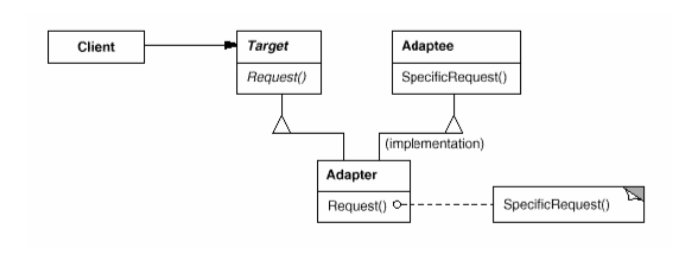
\includegraphics[scale=0.65]{5_1}
    \caption{Padrão \textit{Adapter}}
    \label{figura1}
\end{figure}
			
O padrão é importante para o projeto pois é necessário adaptar as diversas respostas obtidas das diferentes interfaces de cada uma das LMSs integradas ao sistema, para que seja possível que a interface cliente os utilize. Sendo assim, foram implementados um \textit{adapter} para cada recurso diferente previsto na aplicação.

\begin{itemize}
    \item \textit{CourseAdapter}: para disciplinas e cursos;
    \item \textit{EventAdapter}: para eventos;
    \item \textit{FileAdapter}: para arquivos;
    \item \textit{TopicAdapter}: para tópicos;
    \item \textit{AuthenticationAdapter}: responsável pela autenticação em cada um dos serviços integrados;
\end{itemize}

Sozinho este padrão não solucionava todo o problema. Como é preciso lidar com diversas interfaces diferentes, uma para cada LMS, tais classes precisariam ser modificadas toda vez que um sistema LMS novo fosse integrado. Pensando nisso, os \textit{adapters} foram combinados com um outro padrão, o \textit{Strategy}, que passa a cuidar da lógica de adaptação. Os \textit{adapters} recebem como parâmetro a LMS e define a \textit{strategy} correta para adaptação.

\subsection{Padrão \textit{Strategy}}

A intenção do padrão \textit{Strategy}, também conhecido como \textit{Policy}, é definir um grupo de algorítimos, encapsular cada um deles, e permitir que eles sejam permutáveis. Ou seja, permite que a lógica varie dependendo do cliente que precisa utilizá-la.	

\begin{figure}[H]
    \centering
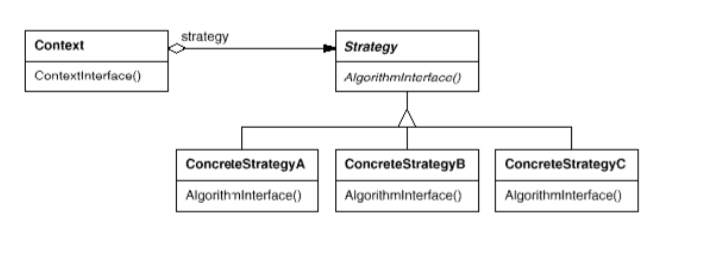
\includegraphics[scale=0.65]{5_2}
    \caption{Padrão \textit{Strategy}}
    \label{figura2}
\end{figure}

As \textit{strategies} do projeto foram idealizadas para serem implementadas isoladamente em cada módulo dos serviços integrados. E assim as classes \textit{adapters} poderíam trocar as estratégias de adaptação das interfaces baseado na chamada do cliente. Por isso, para cada um dos módulos foi preciso implementar uma \textit{policy} para cada recurso, da mesma forma que os adaptadores.

\begin{itemize}
    \item \textit{CourseStrategy}: para disciplinas e cursos;
    \item \textit{EventStrategy}: para eventos;
    \item \textit{FileStrategy}: para arquivos;
    \item \textit{TopicStrategy}: para tópicos;
    \item \textit{AuthenticationStrategy}: para a autenticação;
\end{itemize}


\section{Client-side}
\label{sec:client-side}
A aplicação Client-Side, isto é, a parte que será executada no dispositivo móvel do usuário, tem a função de apresentar de forma clara e objetiva as informações trazidas do \textit{Server-Side} através de uma interface de usuário que seja responsiva aos estímulos particulares utilizados em dispovitivos móveis, como o toque na tela, o arraste de objetos e a rolagem do conteúdo com gestos de "puxar" e "empurrar" dos dedos.  Além disso, a disposição do conteúdo deve levar em consideração o tamanho reduzido das telas dos dispositivos, os botões e teclas físicas disponíveis nos diversos tipos de aparelhos, bem como a disponibilidade e o meio de conectividade com a Internet.

Quando se fala de desenvolvimento de aplicativos para plataformas móveis, certamente um dos maiores desafios é lidar com a heterogeneidade em diversos aspectos dos dispositivos alvo. A começar pelo Hardware, temos telas que variam de 3 a 11 polegadas, com resoluções de imagem e densidades de pixels diversas, há também uma vasta gama de tecnologias de rede em padrões sortidos, com grandes variações nas taxas de transferência de dados, partindo dos 14kbps de conexões GPRS até  taxas superiores a 20Mbps em tecnologias como LTE e WiMax. Existem ainda muitos outros fatores importantes, como a capacidade e o tipo de mídia de armazenamento disponível, a quantidade e disposição dos botões físicos e funções correspondentes dentre os distintos fabricantes, a infindável variedade de hardwares de geolocalizadores, acelerômetros, bússulas, câmeras, entre outros.

A julgar pela diversidade apresentada no hardware já se pode constatar a necessidade de um ferramental próprio para lidar com este desafio. No entanto, divergências mais impactantes são apresentadas quando olhamos a fundo as possibilidades existentes na camada de Software dos dispositivos.
Analisando apenas as possibilidades de sistemas operacionais, constatamos a existência de uma grande quantidade de opções, sendo as principais o Android, o iOS, o Windows Phone \cite{report:idc}, além de outras distribuições menos representativas, ou que já perderam grande parte do seu mercado ao longo da última década, como Symbian, Blackberry e WebOS. 

Cada um dos Sistemas Operacionais traz junto consigo uma série de particularidades que devem ser consideradas ao ser escolhida como alvo de um projeto de aplicativo.
De todas essas particularidades, o tamanho da comunidade de usuários que será contemplada certamente exerce grande influência na escolha do Sistema Operacional que executará o aplicativo.
Outro grande fator a ser considerado é a plataforma de desenvolvimento associada, cada qual com suas respectivas linguagens e ambientes de programação de diferentes custos de propriedade, suas respectivas lojas, custos e regras de distribuição impostos pelos seus fabricantes.


Foi necessário uma análise entre os tipos de aplicativo móvel possíveis de ser desenvolvidos para contornar o problema da alta heterogeneidade dos dispositivos de forma que fosse possível oferecer, com custo de desenvolvimento e qualidade satisfatórios, o aplicativo para a maior parcela possível de usuários dentro da comunidade alvo do projeto. Abordaremos estes diferentes tipos de aplicativo e exploraremos suas vantagens e desvantagens na sessão seguinte e apresentaremos a solução encontrada para o problema relatado.


\subsection{Abordagens de desenvolvimento de Aplicativo Móvel}

\begin{itemize}
    \item Aplicativos Nativos - São específicos para uma determinada plataforma móvel, como iOS ou Android, são construídos diretamente sobre os serviços disponibilizados pela plataforma móvel, expostos através de um conjunto de \textit{Interfaces de Programação de Aplicação (API)} \cite{book:fling}. Utilizam as ferramentas de desenvolvimento e linguagem específicas que as respectivas plataformas suportam \cite{article:malovolta}. Por exemplo, Xcode e Objective-C são suportadas pelo fabricante para desenvolver para iOS, e o Eclipse e a linguagem de programação Java são recomendados para o desenvolvimento para Android. Aplicativos nativos acessam geralmente executam de forma mais fluída por ter melhor desempenho no acesso às funções nativas do dispositivo \cite{article:corral}. Podem trazer uma sensação de usabilidade mais prazerosa, especialmente para requisitos de alto desempenho, como aceleração gráfica por hardware e leitura de sensores em sistemas de tempo real.
    \item Aplicativos Web ou Webapps: Usam as tecnologias web padrão, HTML5, JavaScript e CSS \cite{article:rahul}. Nesta abordagem escreve-se o código uma única vez e o aplicativo pode ser executado em qualquer plataforma. Apesar dos desenvolvedores poderem criar aplicativos sofisticados com apenas HTML5 e JavaScript, existem algumas limitações vitais \cite{article:rahul}\cite{article:spyros}, especificamente o armazenamento offline seguro e o acesso às funcionalidades nativas dos dispositivos, como câmera, calendário, contatos, sensores, hardware de geolocalização, etc.
    \item Aplicativos Híbridos: Esta proposta torna possível incorporar Aplicativos Web dentro de uma fina camada recipiente nativa, combinando os elementos dos Aplicativos nativos e Webapps. A maior parte do aplicativo é construído usando tecnologias web compatíveis com todas plataformas, tais como HTML5, CSS e Javascript - as mesmas línguas usadas para escrever aplicativos web. No entanto, algum código nativo é utilizado para permitir que o aplicativo acesse funcionalidades mais específicas do dispositivo e produza uma experiência de usuário mais refinada. A vantagem desta abordagem é clara: apenas uma porção do código nativo tem de ser re-escrito para o aplicativo funcionar adequadamente sobre os diferentes tipos de dispositivos disponíveis \cite{book:wargo}, se tornando mais rápido e mais fácil de desenvolver que aplicativos nativos \cite{article:ibm}.
\end{itemize}

\pagebreak

\begin{table}[h]
\centering
\caption{Vantagens das abordagens de desenvolvimento de aplicativos móveis \cite{article:swot}}
\begin{tabular}{p{.10\textwidth}|p{.90\textwidth}}
Web & \begin{minipage}{5in}
      \vskip 4pt
      \begin{itemize}
        \item Capacidade de construir uma única vez e implantar todas plataformas
        \item Distribuição Centralizada
      \end{itemize}
      \vskip 4pt
    \end{minipage} \\ \hline
Híbrido & \begin{minipage}{5in}
      \vskip 4pt
      \begin{itemize}
        \item Capacidade de construir uma única vez e implantar todas plataformas
        \item  Custos de desenvolvimento e manutenção reduzidos
        \item Tempo de lançamento reduzido\\ Segurança e gestão do aplicativo aprimorados\\ Desenvolvimento por pessoas com a mesma experiência (HTML5, CSS3, JavaScript)
        \item Acesso as APIs Nativas\\ Distribuição por Loja de Aplicativos
        \item Processamento impulsionado pelo hardware do dispositivo
        \end{itemize}
      \vskip 4pt
    \end{minipage} \\ \hline
Nativo & \begin{minipage}{5in}
      \vskip 4pt
      \begin{itemize}
        \item Melhor desempenho
        \item Rápida adaptação para mudanças no sistema operacional
        \item Controle total do dispositivoSegurança e Gestão de Aplicativos Aprimorados
        \item Acesso as APIs Nativas
        \item Distribuição por Loja de Aplicativos
        \item Processamento impulsionado pelo hardware do dispositivo
      \end{itemize}
      \vskip 4pt
    \end{minipage}
\end{tabular}
\end{table}

\pagebreak




\begin{table}[h]
\centering
\caption{Desvantagens das abordagens de desenvolvimento de aplicativos móveis \cite{article:swot}}
\begin{tabular}{p{.10\textwidth}|p{.90\textwidth}}
\multicolumn{1}{r|}{Web} & \begin{minipage}{5in}
      \vskip 4pt
      \begin{itemize}
        \item Sem acesso as APIs nativas
        \item Sem modo Offline
        \item Processamento não pode ser impulsionado pelo hardware do dispositivo
        \end{itemize}
      \vskip 4pt
    \end{minipage} \\ \hline
Híbrido & \begin{minipage}{5in}
      \vskip 4pt
      \begin{itemize}
        \item Funções nativas específicas podem estar ausentes em algumas plataformas e exigir codificação nativa
        \item Adaptação lenta a mudanças do sistema operacional
        \item Inadequado para requisitos de alta performance
        \end{itemize}
      \vskip 4pt
    \end{minipage} \\ \hline
Nativo & \begin{minipage}{5in}
      \vskip 4pt
      \begin{itemize}
        \item Cada plataforma requer o desenvolvimento independente por times de diferentes especialidades técnicas
        \item Requer teste de plataforma específico
        \item Suporte reduzido e menor oferta de desenvolvedores dependendo da plataforma
        \end{itemize}
      \vskip 4pt
    \end{minipage}
\end{tabular}
\label{my-label}
\end{table}

Considerando o escopo das funcionalidades do aplicativo proposto por este projeto, foi constatado que a maior parte das funcionalidades são relativas a apresentação de conteúdo e que não demandam recursos de alto desempenho para seu bom funcionamento \cite{article:malovolta2}. Soma-se a esta constatação, que promover o acesso a maior parcela possível da comunidade alvo é de suma importância para a proposta deste projeto, portanto todas as plataformas majoritárias devem poder ser atendidas. Por último, é desejavel que alguns recursos nativos estejam disponíveis, como sincronização de informações de acordo com o tipo de conexão disponível, notificações do dispositivo para alertar sobre novos conteúdos e acesso ao sistema de arquivos para armazenamento automático de materiais disponibilizados no aplicativo. Desta forma, a solução Híbrida é a opção mais adequada para a implementação da proposta.

Dentre as tecnologias disponíveis para desenvolvimento móvel híbrido, a ferramenta escolhida para este trabalho, pela sua facilidade de uso, menor custo de desenvolvimento \cite{article:ibm} e que contempla os requisitos desejados é o framework de desenvolvimento móvel, Ionic.


\subsection{Framework de desenvolvimento móvel Ionic}

Para a implementação do aplicativo foi utilizada as largamente difundidas tecnologias WEB tradicionais, o HTML5, o CSS e a linguagem de programação Javascript.

Para que o aplicativo possa ser disponibilizado através de pacotes compilados para dispositivos móveis de diferentes plataformas, como iOS, Android ou Windows, foi utilizado o framework de desenvolvimento de aplicativos móveis híbridos Ionic.

O Ionic incorpora e integra outras tecnologias bastante populares no desenvolvimento web e móvel. Destacaremos dentre elas as seguintes:

\begin{itemize}
    \item O Apache Cordoba, responsável por intermediar o acesso da aplicação escrita em Javascript aos recursos nativos do aparelho, como sistema de arquivos, wi-fi, rede móvel, geolocalização, entre outros.
    \item O AngularJS, um framework Javascript para execução de Single Page Applications, construídas sobre o padrao Model-View-ViewModel
\end{itemize}

A seguir apresentaremos os conceitos chaves destas partes e como elas interagem entre si.



\subsection{\textit{Apache Cordova}}
O \textit{Apache Cordoba} é o \textit{framework} de desenvolvimento de aplicativos móveis híbridos mais popular da atualidade \cite{article:palmiere}, foi criado em 2008 pela Nitobi sob o nome de Phonegap, posteriormente adquirido pela Adobe. A ferramenta cria uma camada recipiente nativa, como uma "casca", para aplicativos escritos em tecnologias Web tradicionais com a finalidade de construir um  aplicativo multi-plataforma.
Com o Apache Cordova é possível gerar um único \textit{baseline}, ou seja escrever um único código-fonte e compilar para todas as principais plataformas, como Android, iOS, Windows Phone , Blackberry, dentre outras.
O código nativo gerado pelo Apache Cordova, permite chamadas aos recursos nativos dos dispositivos nas diversas plataformas de forma otimizada [Apache, Cordova], sem a necessidade de conhecer as interfaces nativas específicas de cada plataforma ou codificar em sua linguagem nativa, como Objective-C ou Java, por exemplo, podendo assim reduzir os custos do projeto \cite{article:tian}.

A arquitetura por trás do Apache Cordova é apresentada na figura \ref{cordova}. 

Na tabela \ref{recursos_suportados_cordova} podemos ver todos os recursos suportados atualmente pelo Apache Cordoba nas diversas plataformas

\begin{figure}[H]
\centering
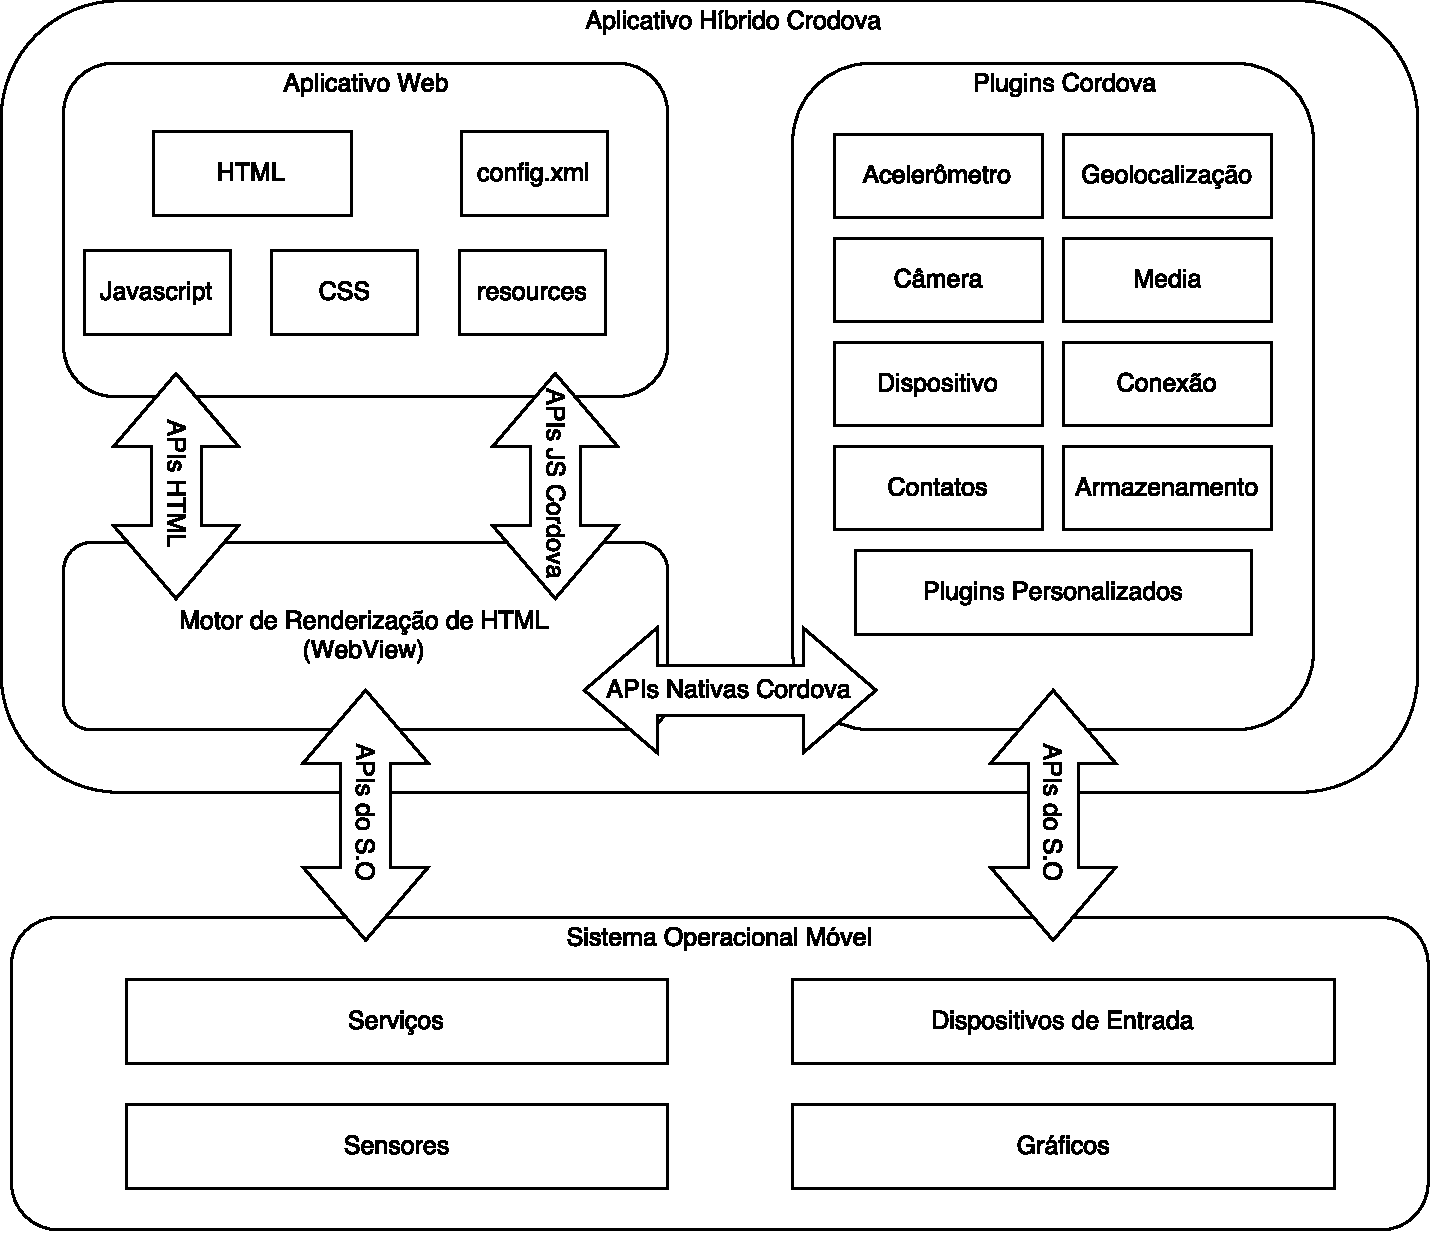
\includegraphics[width=\textwidth]{5_3.pdf}
    \caption{Arquitetura de uma aplicação híbrida com o Apache Cordova. \cite{website:cordova-arch}}
    \label{cordova}
\end{figure}



\begin{table}[h]
\resizebox{\textwidth}{!}{%
\centering
\begin{threeparttable}
\caption{Recursos suportados pela camada nativa do Apache Cordova \cite{website:cordova-platform}}
\label{recursos_suportados_cordova}
\begin{tabular}{rcccccc}
 & Android & Blackberry10 & iOS & Ubuntu & WP8 & Windows(8.1, 10, Phone 8.1) \\
Acelerômetro & \cmark & \cmark & \cmark & \cmark & \cmark & \cmark \\
Situação da Bateria & \cmark & \cmark & \cmark & \xmark & \cmark & \cmark ** \\
Câmera & \cmark & \cmark & \cmark & \cmark & \cmark & \cmark \\
Captura & \cmark & \cmark & \cmark & \cmark & \cmark & \cmark \\
Bússola & \cmark & \cmark & \cmark ** & \cmark & \cmark & \cmark \\
Conexão & \cmark & \cmark & \cmark & \cmark & \cmark & \cmark \\
Contatos & \cmark & \cmark & \cmark & \cmark & \cmark & \cmark * \\
Dispositivo & \cmark & \cmark & \cmark & \cmark & \cmark & \cmark \\
Eventos & \cmark & \cmark & \cmark & \cmark & \cmark & \cmark \\
Arquivos & \cmark & \cmark & \cmark & \cmark & \cmark & \cmark \\
Transferência de Arquivos & \cmark & \cmark * & \cmark & \xmark & \cmark * & \cmark * \\
Geolocalização & \cmark & \cmark & \cmark & \cmark & \cmark & \cmark \\
Globalização & \cmark & \cmark & \cmark & \cmark & \cmark & \cmark \\
Navegador Interno & \cmark & \cmark & \cmark & \cmark & \cmark & \cmark * \\
Media & \cmark & \cmark & \cmark & \cmark & \cmark & \cmark \\
\xmarkification & \cmark & \cmark & \cmark & \cmark & \cmark & \cmark \\
\textit{Splashscreen} & \cmark & \cmark & \cmark & \cmark & \cmark & \cmark \\
Barra de \textit{Status} & \cmark & \xmark & \cmark & \xmark & \cmark & \cmark ** \\
Armazenamento & \cmark & \cmark & \cmark & \cmark & \cmark * & \cmark * \\
Vibração & \cmark & \cmark & \cmark & \xmark & \cmark & \cmark **
\end{tabular}
    \begin{tablenotes}
          \begin{itemize}
              \item[\cmark] 
              suportado
              \item[\cmark*] 
              suportado com limitações
              \item[\cmark**] 
              suportado em algumas versões do S.O. 
              \item[\xmark]  
              não suportado
          \end{itemize}
    \end{tablenotes}
\end{threeparttable}
%
}
\end{table}
 
 
\pagebreak
 
\subsection{AngularJS}

AngularJS \cite{website:guidebook} é um framework Javascript de código aberto patrocinado e mantido pelo Google.
"O objetivo do AngularJS é trazer as ferramentas e recursos que estão disponíveis apenas para o desenvolvimento do lado do servidor para o cliente web e, ao fazê-lo, torná-lo mais fácil de desenvolver, testar e manter aplicativos web ricos e complexos” \cite{book:pro_angularjs}.

AngularJS estende o HTML por elementos personalizados, atributos, classes ou comentários, através das chamadas diretivas. Diretivas são marcações em um elemento DOM que dizem ao compilador HTML do AngularJS para anexar um comportamento especial a esse elemento DOM ou até mesmo transformar o elemento DOM e seus filhos. \cite{website:angularjs}

A seguir estão os recursos oferecidos pelo AngularJS: \cite{book:pro_angularjs}
\begin{itemize}
    \item Ligação bidirecional de dados entre as visões e modelos, o que elimina a manipulação do DOM;
    \item Motor de templates incorporado;
    \item Versão reduzida do jQuery chamado jqLite;
    \item Suporte padrão MVC que ajuda a dividir a aplicação em três áreas distintas:
os dados (modelo), a lógica que opera sobre esses dados (controlador) e a lógica que exibe os dados (visão);
    \item Gerenciamento de dependência;
    \item Roteamento de links aninhados que permite que o estado do aplicativo seja codificado na URL, podendo então ser restaurado para o mesmo estado posteriormente;
    \item Serviços integrados para comunicação com servidor RESTful.
\end{itemize}

AngularJS é uma estrutura que pode ser usada para construir aplicações complexas e de alto desempenho no lado do cliente, de uma forma limpa organizada no padrão MVC. A sua maior vantagem é a construção de aplicações que são de fácil manutenção, testáveis, e facilmente extensíveis.

A figura \ref{angularjs} mostra a arquitetura implementada em uma aplicação AngularJS

\begin{figure}[H]
\centering
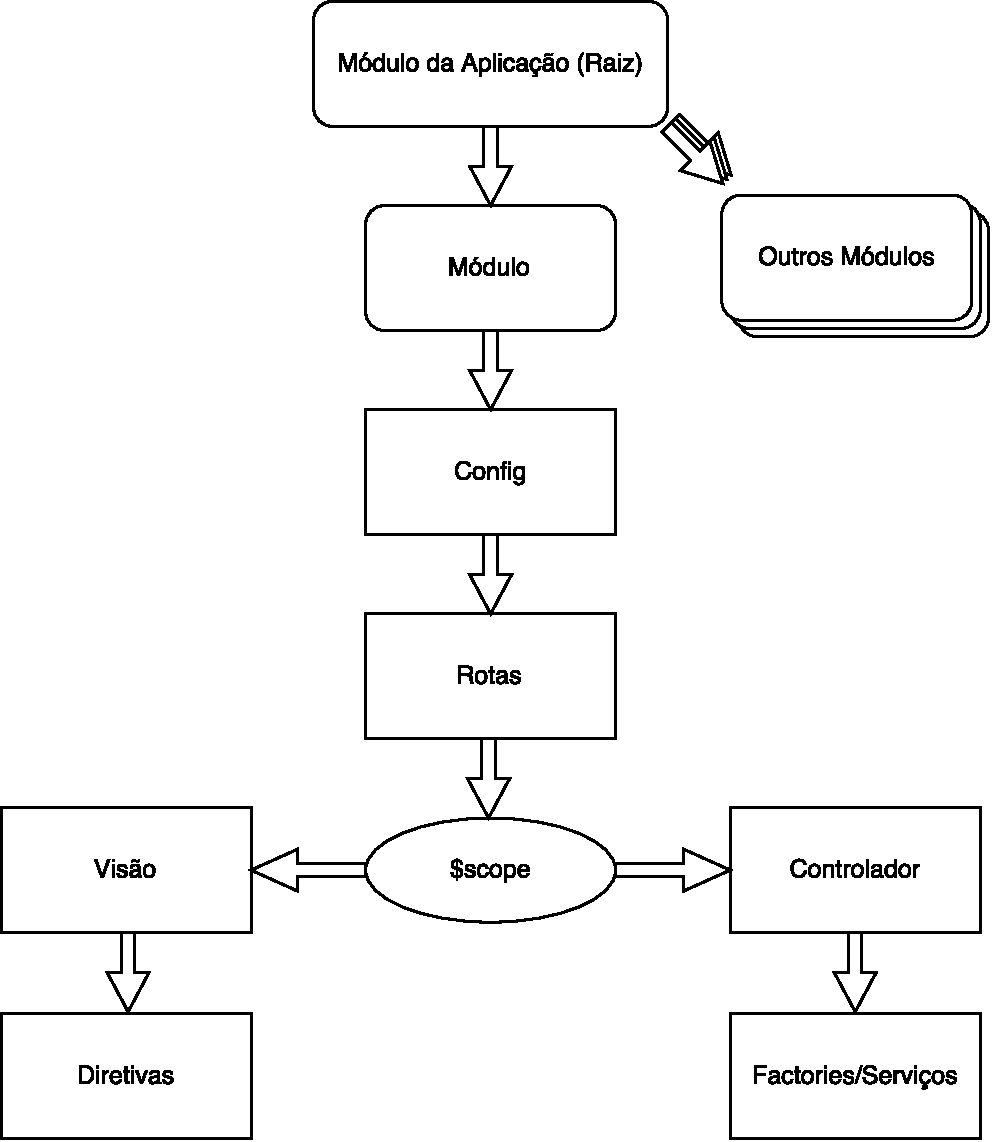
\includegraphics[scale=0.65]{5_4.pdf}
    \caption{Arquitetura de uma aplicação AngularJS \cite{website:angularjs}}
    \label{angularjs}%
\end{figure}




				

				
			
		




%%%%%%%%%%%%%%%%%%%%%%%%%%%%%%%%%%%%%%%%%%%%%%%%%%%%%%%%
%                      Conclusão                       %
%%%%%%%%%%%%%%%%%%%%%%%%%%%%%%%%%%%%%%%%%%%%%%%%%%%%%%%%

\chapter{Conclusão}
\thispagestyle{empty} % retira numeracao da pagina, conforme as normas de apresentacao.

O trabalho final tem como resultado uma aplicação híbrida móvel e uma API integrada com o Conexão UFF. Tais aplicações permitem que os alunos da universidade se conectem ao sistema do Conexão UFF e recebam atualizações de disciplinas, tópicos, eventos e arquivos através da aplicação de uma forma simples e prática.

Considerando os sistemas atuais, é possível identificar melhorias e novas funcionalidades que podem ser implementadas em trabalhos futuros. A principal delas sendo a integração com outras plataformas utilizadas por alunos e professores dentro da UFF. Já que o maior objetivo deste trabalho é facilitar a integração de diversas plataformas diferentes.

Outro exemplo de uma nova funcionalidade seria a implementação de um sistema de mensagens entre alunos através do IntegraUFF. Dessa forma os usuários não precisariam se conectar diretamente através das interfaces de cada plataforma integrada para se comunicar com os outros usuários, e as mensagens ficariam centralizadas em um único local.	

Atualmente o IntegraUFF só permite a sincronização e leitura das informações obtidas das plataformas integradas. Seria desejável que também fosse possível a escrita de informações em tais plataformas através da aplicação. Para a implementação desta funcionalidade é importante considerar que é necessário verificar se as interfaces das plataformas permitem	tal tipo de integração. 

Em relação as melhorias de funcionalidades já existentes, o IntegraUFF hoje já possui uma listagem de eventos na qual é possível marcá-los na agenda padrão do celular. Seria interessante extender esta integração para que o calendário fosse exibido de dentro do aplicativo e/ou os eventos pudessem ser marcados na agenda automaticamente. E para os arquivos, uma integração com o serviço do \textit{Dropbox} \cite{website:dropbox}, permitindo que os alunos enviem os arquivos para a nuvem, e se possível que isso fosse feito de forma automática. 
			
O IntegraUFF é um projeto de código aberto, tanto a sua parte mobile quanto o servidor. Os códigos podem ser obtidos através dos links https://github.com/tiagocandido/client-side-integra-uff, para a aplicação móvel, e https://github.com/tiagocandido/server-side-integra-uff, para o servidor. 		



% %%%%%%%%%%%%%%%%%%%%%%%%%%%%%%%%%%%%%%%%%%%%%%%%%%%%%%%%
%          Sugest�es para trabalhos futuros            %
%%%%%%%%%%%%%%%%%%%%%%%%%%%%%%%%%%%%%%%%%%%%%%%%%%%%%%%%

\chapter{Sugest�es para trabalhos futuros}
\thispagestyle{empty} % retira numeracao da pagina, conforme as normas de apresentacao.

Com base no trabalho desenvolvido, diversas vertentes de trabalhos futuros podem ser identificadas.
%
Tais vertentes, assim como trabalhos individuais em cada vertente, podem ser listados e resumidos.
%
Dessa forma, novas pesquisas podem ser sugeridas, dando continuidade ao trabalho em quest�o.


%%%%%%%%%%%%%%%%%%%%%%%%%%%%%%%%%%%%%%%%%%%%%%%%%%%%%%%%%%%%%%%%%%%
%                  Referências Bibliográficas                     % 
%%%%%%%%%%%%%%%%%%%%%%%%%%%%%%%%%%%%%%%%%%%%%%%%%%%%%%%%%%%%%%%%%%%

\begin{thebibliography}{10}
\addcontentsline{toc}{chapter}{Referências Bibliográficas}

\thispagestyle{myheadings}

\bibitem{norma:esjo2005}
        {Abreu, Estela dos Santos e Teixeira, José Carlos Abreu. 
        \textit{Apresentação de Trabalhos Monográficos de Conclusão de Curso, 8a. edição revisada}, 
        EdUFF, 2005.}

\bibitem{website:ctan}{\textbf{CTAN} (Comprehensive TeX Archive Network), \textit{http://www.ctan.org/}.}
% Este site é referência mundial para materiais relacionados ao TeX e LaTeX.

\bibitem{livro:circuit}{JOHNS, David A. and MARTIN, Ken. \textit{Analog Integrated Circuit Design}, 
John Wiley \& Sons, Inc., 1997.}

\bibitem{book:signal}{MITRA, Sanjit K. , \textit{Digital Signal Processing - A Computer-Based Approach.}, 
The McGraw-Hill Companies, Inc., 1998.}

\bibliographystyle{plain}
\bibliography{bibfile}

\end{thebibliography}

\end{document}


